\chapter{pySpectrum: an Object-Oriented Tool for Batch Processing of Newly Developed Spectroscopic Techniques}
\section{Introduction}\label{sec:writeup_software_intro}
\outlineblank{subsection}
\outlineblank{subsubsection}
In this publication,
    we present the implementation
    of a strategy for spectroscopic data processing.
While motivated by our own research into DNP,
    we believe the resulting strategy and libraries
    should be useful to researchers in a variety of spectroscopic fields.
We provide software to process DNP data coming from common commercial platforms,
    however, we the code also provides a sufficiently robust and flexible
    base to routinely and directly interface with home-built instrumentation,
    as we also demonstrate.
This software also supports a variety of interfaces;
    the interface we favor, and have most fully developed,
    involves direct generation
    of a pdf-format laboratory notebook;
    however, display in the format of a graphical
    user interface (GUI) is also possible,
    with the integration of the appropriate code.
\paragraph{overview}
Until recently,
    spectroscopists had to choose between two types of programs.
High-level
    programs have been designed for optimally performing specific tasks
    very well or in with a very user-friendly interface.
More versatile software,
    such as Matlab, and Mathematica offer the opportunity
    to deal with the data in more detail,
    and offering a great deal of both control and automation in data processing.
However,
    this comes at the expense not only of user friendliness,
    but often with a significant amount of coding.
Most recently,
    open-source libraries for the scripting language Python have
    offered similar capabilities.
However, Python offers a distinct advantage by being {\it modular} and {\it object-oriented}.
We use these benefits to our advantage in a novel way
    in order to attempt to bridge the gap between these two extremes.
We take advantage of the modular, object oriented nature of Python
    to build up a scripting language that should require
    less lines of code and address the data in a more natural way.
In turn, end developers in specific labs or companies
    can more easily build user-friendly applications
    out of these scripts.
\paragraph{structure}
Our strategy follows two key directives:
\begin{itemize}
    \item we are building an open-source toolbox
    \item we subdivide the code into different ``layers,'' where ``deeper'' layers are targeted for editing by users of increasing technical competence/involvement, and have a more general impact on the function of the end software.
\end{itemize}
The layer strategy is deliberately modeled off the
    design strategy that has naturally evolved
    in the open-source / linux community
    (for a common example
    take the entire OS, which is organized in the following layer format:
    application $\Rightarrow$ GUI toolkit $\Rightarrow$ window manager $\Rightarrow$ display server $\Rightarrow$ daemons $\Rightarrow$ kernel).
Applying such a strategy to a far less ambitious
    project, such as that of analyzing spectroscopy data
    allows different users to contribute to the future development
    of each such layer, or even to creating new layers.
In the code presented here,
    one layer provides several processing functions commonly used in DNP,
    while a deeper layer can handle the reading of NMR data files (i.e. Bruker or Kea format),
    or can pull data directly from instruments,
    such as oscilloscopes.
The deepest layer we present 
    here (the nddata class and related functions,
    discussed below),
    abstracts $N-$dimensional into 
    a new/specialized type of object,
    so that one can manipulate it in a more
    transparent way, with fewer lines of code.
The entire code rests on top of multiple layers
    of general mathematical libraries previously created by the open
    source community.
\ntd{show a diagram with labeled classes/modules here!}
\paragraph{spectroscopy layer}
We place special emphasis on the layer responsible for
    storing the spectroscopic data.
By taking advantage of the object-oriented nature of python,
    we can bind together the data describing the spectrum
    with information about its axes, errors, and units.
We keep track the various dimensions of multi-dimensional data
    by providing sensible labels for the various dimensions.
We then define a series of abstract routines that handle the resulting
    bundle of data (i.e. object) in an intuitive way.
For instance, relabeling of the axes after Fourier transformation,
    propagation of the error,
    determination of the units,
    and labeling of plot axes,
    all happens {\it automatically},
    without the need for further coding.
We can also slice out pieces of a spectrum by frequency range in a simple way,
    and we can handle highly multi-dimensional data
    (such the separately stored phase cycles of multi-dimensional NMR spectroscopy)
    easily.
This object-oriented design forms the core of our strategy,
    which proves to have many benefits.

\section{Review of relevant tools}
\ntd{be sure to pull relevant stuff from installation first}
\subsection{Latex}
\subsection{Python}
\subsubsection{Numpy}
\subsubsection{Scipy}
\subsubsection{PyTables}
\subsubsection{Qt}
\subsection{Revision Control Systems}
Revision (or version) control systems
    are used to keep track of the history of files,
    on a change by change basis.
In particular, they are designed for two purposes we find useful:
\begin{itemize}
    \item In the event that data is overwritten, or code is broken,
        they allow one to easily compare to or revert to an earlier
        version of the data/code.
    \item They allow two or more users to work simultaneously and seamlessly
        on a project, whether it be data acquisition, coding, or paper writing.
\end{itemize}
We use subversion (SVN) to distribute an updated version of our code,
    and so you will at the very least need
    to use the TortoiseSVN program (below)
    to download it;
    for more advanced users, we recommend Git (also described below).
In addition to this purpose,
    we also highly recommend
    setting up a latex-based lab notebook
    on a revision control system.
This allows one to distribute the notebook
    to various computers, while also maintaining the benefits noted above.
\paragraph{Git}
Another revision control system,
    known as Git, is far more powerful than SVN, and does not require
    a central server.
It \textit{can} also pull from and push to SVN repositories.
For the experienced user, we recommend its use over that of SVN.
However, as it is substantially more advanced than SVN,
    we cannot do a proper introduction
    justice here,
    and instead refer the reader to the ProGit online book,
    the Git user manual,
    and the following list of useful ``survival commands''
\begin{lstlisting}
    # this is after installing msysgit on windows
    #       you have to be sure to select the bash shell
    #       context menu option when installing!!!
    # make a new folder
    # right click --> git bash here
    # note that I could actually do "git clone" rather than this,
    #       which should also (unlike this procedure), clone
    #       more than one branch.
    #       However, this is more instructive 
    git init # this sets up the local repository
    git sources add origin gitolite@franck.privatedns.org:notebook # this adds the remote repository as a remote source called "origin" (which is the default)
    git remote show origin # this shows what's on the remote repository
    git pull origin master # this pulls down "master" (the usual name of the main branch) from "origin"
    git branch # this just shows what branches are on the remote branch
    git remote show origin # now we should see how the local branches are tracking the remote branch
    git branch -a # this shows all branches, both remote tracking branches and local branches
    git gui # this opens the gui to track my changes
    # this is good both for scanning for changed files,
    # staging those changes for committing,
    # as well as committing and pushing
    # additionally, you can use it to explore branch history,
    # where you can right-click to create named tags
    git checkout -b mynewbranchname # create a new branch
    # based at the point in history you currently have
    # checked out, then check out that branch
    git checkout mypreviouslycreatedbranchname # make
    # the working copy look like the last commit in
    # previouslycreatedbranchname
    git checkout mytagname # this is how I check out
    # (for instance to test) a previous revision
    # note you can also specify by date/number of revisions
    # back, etc (see git user manual or pro git book)

    # analogs of svn
    git svn clone # this is like an svn checkout
    git svn rebase # this is like "svn update"
    git svn dcommit # this is like "svn commit"
    gitk # good for exploring the history of a single file
    # and marking named tags (right click) 
    git bisect # good for finding where the code broke,
    # so you can make a new branch at that point, or revert that
    # change (see the git user's manual for a good example of
    # git bisect)

    # to understand analog of svn merge -r 303:295, look at
    # git revert and git cherry-pick
\end{lstlisting}
Of course, gvimdiff works well for vim users.
Meld looks nice for non-vim users, but not well supported for windows.
Perforce visual merge tool looks good:
\url{http://www.perforce.com/product/components/perforce_visual_merge_and_diff_tools}
Or, for a mixture check out the following sophisticated option from
\url{http://stackoverflow.com/questions/9032133/multiple-diff-tools}
that uses the following external merge tool:
\begin{lstlisting}[mathescape=false,language=bash]
#!/bin/bash

# Parameters from git:
# 1    2        3       4        5        6       7
# path old-file old-hex old-mode new-file new-hex new-mode

CONTINUE=1
while [ $CONTINUE == 1 ]
do

# Present Options
echo "1. P4Merge"
echo "2. Unix diff"
echo "3. Cancel"
echo -n "Choose diff tool[1]: "

# Read in user choice
read -n 1 OPTION

# move down a line
echo ""

# if user didn't enter a choice default to 1
if [[ $OPTION == "" ]] ; then
OPTION="1"
fi

# Launch diff tool based on OPTION
case $OPTION in
1) /Applications/p4merge.app/Contents/MacOS/p4merge "$2" "$5" ; CONTINUE=0 ;;
2) diff "$2" "$5" ; CONTINUE=0 ;;
3) exit ;;
*) echo "\"$OPTION\" is not valid " ;;
esac


# This sleep has two purposes
# 1) on an invalid choice it delays the menu just a hair
# 2) keeps this script alive long enough that git will not just move onto the next file
#    instantly if diffing multiple files.
sleep 1

done
\end{lstlisting}

Either is most easily set up with an external diff
    wrapper that looks like the following:
\begin{verbatim}
#!/bin/sh

# diff is called by git with 7 parameters:
# path old-file old-hex old-mode new-file new-hex new-mode

"/c/Program Files (x86)/Vim/vim73/gvim" -d "$2" "$5" | cat
\end{verbatim}
\section{Installation}
\subsection{Install required software on Mac}
When I write this, there not a very good free all-in-one Python package for the Mac.
The solution is still straightforward, though it takes a little time for everything to compile.
You should download Xcode, then install the following Python components \textbf{Ryan and Anthony: using which package manager??}
\begin{small}
\begin{multicols}{3}
\begin{enumerate}
    \item Python2.7 or higher, but not Python3
    \item ipython
    \item matplotlib
    \item numpy
    \item pyreadline
    \item pyserial
    \item scipy
    \item sympy
    \item pytables
\end{enumerate}
\end{multicols}
\end{small}
You will also need to download some form of \LaTeX\ distribution \textbf{Ryan and Anthony, please recommend a latex distribution}
\subsection{Install required software on Windows}
%%fakesubsubsection
\outlineblank{subsubsection}
Python(x,y), TortoiseSVN, SumatraPDF, and miktex are all required
    to download the notebook code and generate and view PDF output
    of the data.
All three packages are open source code,
    and
    the official websites where the code can be downloaded can all be found
    with a simple google search.
\paragraph{Python(X,Y)}
First, install python(x,y) from their google code site.
\begin{inplacenotebox}
    This is an excellent python distribution that includes most of
    the dependencies that nddata uses (and which are generally useful for scientific purposes).
    This also includes MinGW, which is a minimal version of the
    GNU C compiler for windows -- this can be used to compile
    C extensions to python, for instance, to communicate with hardware
    (such as our YIG source).
\end{inplacenotebox}
When installing, you should click on the ``Python'' box,
    so that it displays a green check (NOT a grey check).
This installs a variety of useful python libraries,
    including the sympy package, which the nddata library uses.

When you are done with this, open a dos shell (Start Menu $\Rightarrow$ type \texttt{cmd}, or Start Menu $\Rightarrow$ Run Command $\Rightarrow$ type \texttt{cmd}),
    and type \texttt{python}.
It's important that typing this does not lead to an error,
    but rather opens the python interpreter,
    which will say something like ``Python 2.7.2\ldots'' and give you a prompt.
After verifying this, you can just type ``exit()''
\begin{inplacenotebox}
    If, for whatever reason, this does not work,
    you need to set up your windows command path correctly.
\end{inplacenotebox}
\paragraph{TortoiseSVN}
TortoiseSVN, from tortoisesvn.net is a great windows
    client for subversion (svn),
    which we are using to distribute the notebook code and keep
    it up to date.
When installing, be sure to download the correct version (32 bit or 64 bit windows) for your computer, and when installing, you will have to select the command line tools, which are deselected by default.
\begin{inplacenotebox}
If you have Git installed, you do not need TortoiseSVN.
You can just use the ``git svn clone\ldots'' and ``git svn fetch\ldots''
    commands (see above and Git documentation.)
\end{inplacenotebox}
\paragraph{miktex}
Download miktex (latex for windows).
You should configure it to download new packages on an as-needed basis.
\begin{inplacenotebox}
    Sometimes,
    if you've had a miktex installation on your computer for a while,
    for some reason it stops automatically grabbing packages on an as-needed
    basis.
    If this happens, I recommend just uninstalling completely and reinstalling
    again.
\end{inplacenotebox}
\paragraph{SumatraPDF}
Finally, SumatraPDF allows you to recompile a PDF
    file with latex while the PDF is still open
    (Acrobat Reader doesn't have this capability).
You need to install it as well.
\subsection{Install an Editor}
%%fakesubsubsection
\outlineblank{subsubsection}
\paragraph{notepad++}
Any text editor can, of course, edit
    python scripts and latex files.
For Windows,
    we recommend Notepad++ (freeware)
    which supports syntax highlighting (i.e. coloring)
    and the folding of sections of code.
\subsection{Install the notebook code}
%%fakesubsubsection
\outlineblank{subsubsection}
The notebook code itself consists of a set of home-built
    python libraries
    (described through the rest of this document)
    that help you develop code to process the data,
    in addition to some code (described later)
    that allows you to embed such scripts in a latex file.
\paragraph{Download (for novice Windows users)}
Use TortoiseSVN to check out the
    most recent version of the code
    by right-clicking on your desktop,
    or inside any folder
    (it doesn't matter where you install the code),
    and selecting ``SVN Checkout\ldots''
You then need to enter the URL of the repository, which is:
    \\ \url{https://franck.privatedns.org/svn/public\_notebook}
    (pay attention to the https).\\ 
This will create a folder with the code.
You can install future updates to the code
    simply by right-clicking on this folder,
    and selecting SVN update.
\paragraph{Download (On the mac, or Git users)}
Install Git and git-svn (on windows, you can get these from msysgit, on mac you need to download Xcode and then \textbf{I don't know, Ryan and Anthony please remind me}), if you don't already have it.
\begin{inplacenotebox}
If you are already a Git user, congratulations, you are awesome!
This note is for you.
If not, skip this note.

You can add the public notebook as a remote source as follows
    \begin{enumerate}
        \item change to the working directory where you will
            want to import the notebook code and run \texttt{git commit -a} 
            to commit any changes to your working directory.
        \item \texttt{vim .git/config} 
            and add:
    \begin{tiny}
            \begin{verbatim}
[svn-remote "public"]
	url = https://franck@franck.privatedns.org/svn/public_notebook
	fetch = :refs/remotes/git-svn-public
            \end{verbatim}
    \end{tiny}
        \item \texttt{git svn fetch public} 
            (this pulls the history)

        \item \texttt{git branch -t public remotes/git-svn-public} 
            (this creates a local branch called ``public'' that tracks the remote)

        \item \texttt{git checkout public} 
            (this switches to the public branch)

        \item \texttt{git svn rebase} 
            (this is to check that it's up-to-date, and, yes, it is frequently necessary)

        \item \texttt{git checkout master} 
    \end{enumerate}
The ``public'' branch then stores a copy of the public code.
You can pull updated code into the public branch.
Typically, your working code will be in your ``master'' branch,
    and you will then want to (possibly selectively) merge the updates
    from ``public'' into ``master.''
\end{inplacenotebox}
To start a fresh directory called \texttt{public\_notebook} that contains the public notebook code, and where you will run your scripts, run the command
\texttt{git svn clone} \url{https://franck.privatedns.org/svn/public\_notebook}.

In either case, you can then run \texttt{git svn rebase} to update the code when updates are published.
\paragraph{Running the Graphical User Interface (GUI)}
The notebook code comes with a graphical user interface
    (GUI) that allows you to tell the
    code where you keep your data,
    and allows you to select and run processing scripts
    without having to use the command prompt.
Go into the folder where you have installed the notebook code,
    and double-click on script\_gui.py.
This will open a window that looks like this:
\begin{center}
    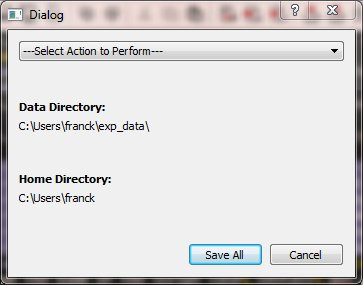
\includegraphics[width=3in]{sketches/script_gui.jpg}
\end{center}
\john{change the title of this box}
It will also open a window with a black background --
    this is for debugging purposes only
    and should be ignored \nts{and will be removed
    later.}
\paragraph{First-time setup}
You should choose a directory
    on your computer
    where you store all of your raw data. 
You can organize your data however you like within this directory,
    but in the following note,
    we recommend an organization
    used by the examples in this document.
\begin{inplacenotebox}
    Typically, it's useful if the data directory
        has a different subdirectory for
        each instrument you use,
        so that you have a directory structure that
        looks something similar to this:
    \begin{itemize}
        \item Data Directory: \verb|c:\Users\Franck\exp_data\|
            \begin{itemize}
                \item \verb|c:\Users\Franck\exp_data\franck_cnsi\|
                \item \verb|c:\Users\Franck\exp_data\franck_hanlab\|
                \item \verb|c:\Users\Franck\exp_data\reference_data\|
            \end{itemize}
    \end{itemize}
    Where, for example, each of these contains WinEPR .spc and .par files,
        as well as an \verb|nmr| subdirectory that contains all
        the NMR data from Topspin.
    In this way, WinSCP/freesshd or another
        file transfer software could be used to synchronize the
        data for a particular instrument with a particular
        directory.
\end{inplacenotebox}
To set the location of your main data directory
    (``exp\_data'' in the example above),
    simply select ``Set Data Directory'' from the drop-down list
    at the top,
    and select the appropriate folder.
If, when quitting the program, you press ``Save All,''
    the script\_gui.py program
    will remember the location of your data directory
    the next time you open it.
    \begin{inplacenotebox}
        Incidentally, this is also the point at which it configures
            everything needed to run large latex file(s)
            that can organize and collect the information from
            several different python scripts.
        \nts{This will be discussed later.}
    \end{inplacenotebox}
\paragraph{Running the example scripts}
Additionally, to run the examples
    you need to retrieve the zip file
    that contains various sets of example data\\ 
    \url{http://franck.privatedns.org/~franck/reference_data.zip}\\ 
and unpack it inside your main data directory,
    so that your data directory has a subdirectory called
    ``reference\_data,'' as shown in the note above.
Once you do this, you can select ``Run Script'' from the dropdown
    list,
    and select ``standalone\_example.py,''
    which is a python script.
Upon hitting OK the program simply hangs for
    half a minute
    \nts{(which will be fixed later)}
    as the script runs.
During this time,
    the python script is reading in your raw FID or
    EPR spectrum data directly,
    applying the procedure described in~\cite{FranckPNMRS},
    and using it generate the final plot of $k_\sigma s(p)$
    and the resulting fit value of $k_\sigma s_{max}$.
The script also generates a set of figures and tables
    that present the data leading up to this final result.
It arranges all these plots and figures inside a latex file
    (if you have already run the script once, it will try to
    overwrite the same tex file, which is usually OK).
\paragraph{Generation of PDF}
When the script is done, it should inform you that it ran without
    errors.
\begin{inplacenotebox}
    If there was some type of data processing error,
        it would show up here, and you could fix it  by modifying the
        python script appropriately.
    Of course, the example script has no such errors,
        so if it fails to run,
        some part of the installation and setup was not completed correctly.
\end{inplacenotebox}
Finally, when you click ``OK,'' latex (specifically miktex's pdflatex)
    will compile the .tex file in order to generate a PDF file,
    which should pop up after a few seconds.
\paragraph{Custom Use}
To process different sets of ODNP $k_\sigma s_{max}$ data,
    you can simply duplicate the example python script
    and edit it
    (all this can be done by right clicking
    within the box where you select the python script.)
While the code can be many lines long,
    modifying it to process a new set of raw data should be easy.
For instance, the standalone\_example code looks like this:\\ 
    \begin{lstlisting}
from h5nmr import *
import textwrap
grab_data_directory()
###########################{{{
# change the following, and if necessary the t1mask line
# below
name = 'dna_cs19_unbound_120418' # replace with the name
# of the experiment
chemical_name = 'dna_cs19_unbound' # this is the name of
# the chemical i.e. 'hydroxytempo' or 'DOPC', etc.
run_number = 120418 # this is a continuous run of data
SL_concentration = 200e-6 # the concentration of spin
# label
dontfit = False # only set to true where you don't expect
# enhancement
extra_t1_problem = True # always start with this false,
# and if it complains, about the number of T1 powers not
# matching with the number of T1 experiments, then turn it
# to True
path = getDATADIR()+'reference_data/nmr/'
search_delete_datanode('dnp.h5',name) # comment this line
# out if you are OK with the script pulling the data from
# previously cached stuff written to the database
###########################}}}
# leave the rest of the code relatively consistent
#{{{ generate the powers for the T1 series
print 'First, check the $T_1$ powers:\n\n'
fl = []
t1_dbm,fl = auto_steps(path+name+'/t1_powers.mat',
    threshold = -35,t_minlength = 5.0*60,
    t_maxlen = 40*60, t_start = 4.9*60.,
    t_stop = inf,first_figure = fl)
print r't1\_dbm is:',lsafen(t1_dbm)
lplotfigures(fl,'t1series_'+name)
print '\n\n'
t1mask = bool8(ones(len(t1_dbm)))
# the next line will turn off select (noisy T1
# outputs) enter the number of the scan to remove --
# don't include power off
if extra_t1_problem == True:
    t1mask[-1] = 0
#}}}
dnp_for_rho(path,name,integration_width = 160,
        peak_within = 500, show_t1_raw = True,
        phnum = [4],phchannel = [-1],
        t1_autovals = r_[2:2+len(t1_dbm)][t1mask],
        t1_powers = r_[t1_dbm[t1mask],-999.],
        power_file = name+'/power.mat',t_start = 4.6,
        chemical = chemical_name,
        concentration = SL_concentration,
        extra_time = 6.0,
        dontfit = dontfit,
        run_number = run_number,
        threshold = -50.)
print r'\subparagraph{Noise test}'
standard_noise_comparison(name)
    \end{lstlisting}
\quad\\ 
Notice the block of code starting with\\ 
    \verb|###########################{{{|\\ 
    and ending with\\ 
    \verb|###########################}}}|\\ 
Only the code within this block
    needs to be modified in order to have
    the script process a new set of data.
(Ideally, it makes sense to create a new script
    for each set of data.)
\nts{Later, we will develop a GUI window
    that changes these parameters.}
The comments (which in python start with ``\#'')
    next to each equation
    inside this block
    should sufficiently explain
    what each parameter means.

Notice the general strategy here:
    more advanced users can write new python scripts
    that process entirely different sets of raw data
    -- for instance a ODNP time course, or a pulsed EPR experiment --
    and then distribute that code,
    while others can simply modify the parameters in the
    parameter block \nts{which again, we can later make
    possible with the GUI} in order to apply that code to
    their data.

The script\_gui.py program can run any python script
    that prints output in a format suitable for a tex file.
All the nddata and associated libraries discussed in the
    remainder of this document can be imported by such scripts;
thus similar python scripts
    can be used to process EPR or even manually acquired
    instrumental data, as well.

The following sections will describe:
\begin{itemize}
    \item how to compile several python data processing
        scripts into an organized latex notebook
    \item how to compile the processed data (which is
        automatically databased) from several ODNP
        experiments into a table or graph containing all
        the data for an experiment
    \item how to understand the details of the underlying
        libraries
        that allow one to write routines for entirely
        new sets of data
        and that take advantage of the
        abilities of objective python programming to
        (among other things)
        \begin{itemize}
            \item automatically label plots
            \item automatically propagate units and
                errors
            \item automatically manipulate axes during Fourier
                transformation
            \item store and retrieve information from the databases
        \end{itemize}
\end{itemize}
\textbf{This is the point to which this writeup is ready
for public consumption.  Stop here.}
\subsection{Further notes for advanced users}
%%fakesubsubsection
\outlineblank{subsubsection}
Unless you are an advanced user (fluent in some type of programming),
    it's probably best to skip ahead
    to ``Installing the notebook.''
\paragraph{\textit{alternative:} manual installation}
Rather than installing Python(X,Y) (if you are crazy),
    you can choose to install a selection of Python packages manually.
All the required packages are
\ntd{grab the list from my notebook}
\ntd{before, on cnsi, I had the following programs installed:}
\begin{itemize}
    \item Python2.5
    \item ipython-0.10
    \item matplotlib-0.99.1
    \item numpy-1.4.0
    \item pyreadline-1.5
    \item pyserial-2.5-rc2
    \item PyUSB-1.5
    \item pywin32-214
    \item scipy-0.7.1
    \item Python 2.6 ipython-0.10 (this should not be required)
\end{itemize}
\ntd{note that sympy and pytables are missing from this list.
However, this should translate into a usable list of required packages.
}
    \paragraph{latexmk}
You also have to create a file in your home directory (in windows the one \textit{above} ``My Documents,'' which is called by your user name) called \texttt{.latexmkrc} with the following code in it
\ntd{here, I should create the directory tex\_build in the svn repo!}
\begin{verbatim}
$pdflatex=q/pdflatex %O -synctex=1 -shell-escape %S/;
$pdf_previewer=q/start sumatrapdf -reuse-instance/;
\end{verbatim}
This sets the pdf viewer to sumatrapdf and tells it to compile the latex file
    with markers for reverse editing and (crucially) sets ``shell escape,''
    a security setting needed to run the latex files.
Note that I tried to set up an aux\_dir or out\_dir,
    but then the python programs get confused about which directory
    they are operating in.

Once you have done this, you can set
    your program to continuously compile and update
    by issuing the following command on the dos prompt:
    \verb|latexmk -pdf -pvc myfilename.tex|
\paragraph{vim}
At this point, we make special mention of
    the text editor vim.
There is a steep learning curve associated with vim.
However, vim is also the most powerful text editor available,
    and will work on any operating system.
In particular, the latex-vim package is particularly useful,
    and can be used to write up equations in latex generally
    as fast as they can be written by hand.\footnote{The surround and align packages \ntd{give site} are highly recommended when using vim as well.
    As part of the notebook svn repository, we have included
        the directory ``vim\_settings,'' which has not only
        a (slightly modified) copy of latex-vim, but also a highly
        tested vimrc file that includes a variety of different features.
    These are not detailed here, and so the file should only be used
        after one has obtained a working knowledge of latex-vim,
        but those familiar with vim will find the <ctrl-D>/ macro
        surprisingly useful for locating phrases with
        printed and hand-edited documents;
        this macro searches for phrases
        based on the start of the words in the phrase $\Rightarrow$
        for instance, typing ``$<$ctrl-D$>$/ On h v c w''
        in edit mode will find ``{\bf On}ly {\bf hi}gh {\bf v}oltage {\bf c}apacitors, {\bf w}ithout\ldots''
    This macro also allows for special characters (also surrounded by spaces):
    ``!'' to position the cursor, ``*'' to find any word, \nts{``**'' to find any number of words};
        of course,
        ``On'', ``h'', ``v'', ``c'', and ``w'' above are actually
        regular expressions, and can be extended accordingly.}
Also, by setting the top radio select in
    ``TortoiseSVN $\Rightarrow$ settings $\Rightarrow$ external programs $\Rightarrow$ diff viewer''
    to ``External,'' and entering something like (depending on your exact install path)
    \verb|C:\Program Files (x86)\Vim\vim73\gvim.exe -d|,
    you can use the vim diff tool to compare different versions of code
    in TortoiseSVN;
    vim is far superior to TortoiseSVN's native tool for doing so.
\paragraph{latexdiff}
\nts{
This is a very nice program that allows you to generate
    Microsoft-Word-like displays of differences between files.
Though we have a very good idea of how to do better in python,
    which would allow us to actually exceed Microsoft Word's capabilities
    by showing which sections get moved where.
If you install the command-line tools for TortoiseSVN,
    you can use }\begin{verbatim}latexdiff-vc -rVERNUMBER --force yourtexfile.tex|\end{verbatim},
    \nts{where VERNUMBER is the version you wish to compare to.
This is truly amazing,
    allowing you to show differences between whatever version
    of the file you like.
However, in order to get it to work on windows, you need to make
    the following changes:
    }
    \begin{description}
        \item[perl] be sure you have installed active-state perl (above)
        \item[patch] download and get the gnuwin32 version of patch
            (get the ``complete package'' file, and install it,
        \item[add patch to command line] 
            add \verb|C:\Program Files (x86)\GnuWin32\bin| to
            the path (search for ``path,'' and system variables will pop up, add to the semi-colon separated list given by the ``path'' variable.)
    \end{description}
    \ntd{this still doesn't seem to work!!! (b/c of stupid little shit)}
\paragraph{SumatraPDF}
Sumatra PDF allows you to recompile a pdf
    with latex while it has it open.
It will update on the fly.
\paragraph{Make directories}
The GUI also does the following:
\begin{itemize}
    \item If you are running the .py files indepedently on the command line,
        you need to create an ``auto\_figures'' directory
        inside the public notebook directory that TortoiseSVN created;
        this is where all automatically created figures are stored.
    \item Also, you need to create a file called ``.datadir'' in the directory,
            and point it at the directory that contains your data.
\end{itemize}
\paragraph{Running a basic python script}
Now, we will operate in the most basic mode by simply running
    a python script to process our data.
\nts{
We can do this
    by opening a terminal (Mac/Linux) or Start Menu $\Rightarrow$ cmd
    under windows,
    changing directories (\texttt{cd}) to our public notebook directory,
    and entering the command
\texttt{python example\_dnp\_data.py > example\_dnp\_data.tex}
}
\ntd{be able to execute commands like this from the gui}
This will process a DNP dataset.
Since DNP data is rather complex,
    we want to generate plots for each step in the processing,
    and also output various tables with $T_1$ times, etc.
The easiest way of compiling all this information
    is in a PDF file, which we generate with Latex code.
So, the python program above generates the latex code
    in the file ``example\_dnp\_data.tex.''
In order to view this in a friendly format,
    we can simply run \texttt{pdflatex example\_dnp\_data.tex}.
\ntd{insert stuff here}
\subsection{Running inside a latex file}
%%fakesubsubsection
\outlineblank{subsubsection}
\paragraph{latexmk}
In addition, you can install latexmk, which repeatedly checks for
    changes to the files and re-compiles the latex file as necessary.
To use this, you will need Perl; you can download and install
    ActiveState Perl.
\nts{We may actually replace this with home-built code,
    and this is not required right off.}
\paragraph{random}
If at any point you see something like ``For the code to work, you need to run pdflatex with shell escape!'', \ntd{for this to work, I will need to include the scripts directory and the error message file in the svn distribution.}
    it's because you need to be sure that you are calling pdflatex with the ``--shell-escape'' flag -- this can be configured by setting the ``compiler'' options in programs such as TeXworks, TeXnicCenter, etc.
\paragraph{included program}
\nts{The easiest way to get started is to use the included
    compile\_latex.py script,
    which compiles with default options.
It also continuously checks for updates to your
    data, rebuilding only as necessary
    (similar to latexmk, but with less options and without requiring perl)
    and allows you to compare changes you have made to a document
    at various points in time (duplicating the functionality of latexdiff-svn more simply and robustly, and also without requiring perl).}
\paragraph{Set SumatraPDF inverse search}
Also, if you use latexmk after using the notebook installer program,
    as described here,
    you can open one of your PDF's, go to
    ``Settings $\Rightarrow$ Options,''
    and select the editor of your choice
    (we recommend notepad++ for the beginner)
    under ``set inverse search command.''
From then on, whenever you double click in a properly compiled PDF,
    your editor will open at the correct line of latex source code.
\paragraph{latexmk combined with synctex}
For windows, the combination of notepad++ and sumatraPDF,
    used in combination with latexmk (see latexmk and
    sumatraPDF installation below),
    works well for editing tex files.
Note that, if you compile your latex files with synctex 
    (as given in the latexmk instructions here)
    sumatraPDF will open your text editor of choice when you double-click
    on the relevant section of text -- see further information
    in the relevant sections below.
\section{Examples}\label{sec:writeup_software_examples}
Note that in the following examples, long descriptive variables names are chosen for more legible code.
The length of the code increases accordingly.
\outlineblank{subsection}
\subsection{tau protein time courses}
\subsubsection{$E$ vs. $t$}
\begin{lstlisting}
import interptau
#make a list to store the figure info in
#start with the parameter that I want to generate the svg files
fl = [{'gensvg':True}]
# first, use put all the file information into a record array
#   record arrays are a useful way of storing labeled/spreasheet-type
#   data in python (we could actually read in a .csv file here, if we wanted to)
file_info = csv2rec('for_anna_processing.csv')
print lsafen(file_info)
print file_info.tolist()
print shape(file_info)
for j in range(0,len(file_info)): # loop over the different records
    thisfile = file_info[j]
    # first, just go ahead and integrate the data
    data,fl = integrate(str(thisfile['file_name']),
            thisfile['expno'],
            first_figure = fl, # this passes the information necessary to plot
            integration_width = 75,
            dimname = r'exp #',
            pdfstring = 'run%d'%j)
    nextfigure(fl,'enhancements') # set any plots to go into
    # the file labelled ``enhancements.''
    # Now, since the first experiment is unenhanced signal, we first
    data /= data[r'exp #',0:1] # normalize to find enhancements, then
    data = data[r'exp #',4:] # anna says to throw out the first three scans
    data.getaxis(r'exp #')[:] -= 4 # set the first point to time 0
    # convert the experiment number axis into a time axis using our conversion
    # next, I need to convert from experiments to seconds
    data.rename(r'exp #','t')
    nexp = data.getaxis('t').max()
    #data.setaxis('t',data.getaxis('t').copy()*double(thisfile['total_min'])*60/nexp)
    data.setaxis('t',double(thisfile['total_min'])*60)
    data.set_error(None) # finally, let's just ignore the error bars for now
    data = 1.-data # convert to 1-E
    plot(data)
    t_axis = data.getaxis('t')
    ylabel('$1-E$')
    xi_for_timecourse = double(array([thisfile['xi%d'%k] for k in r_[1:4]+1])) # pull xi1,xi2,xi3,and xi4
    xi_before = double(r_[thisfile['xi1']]) # pull xi1,xi2,xi3,and xi4
    print lsafen('debug xi_for_timecourse',xi_for_timecourse)
    xi = nddata(xi_for_timecourse,[-1],['t'],axis_coords = [r_[0.,100.,14*60.]*100]) # pull the information
    nextfigure(fl,'taucoarse')
    tau_coarse = xi.copy()
    tau_coarse.data = interptau.interptau(tau_coarse.data,14.5,simple = True)
    tau_before = interptau.interptau(xi_before,14.5,simple = True)
    c = plot_color_counter()
    plot(r_[0.],tau_before/1e-12,'x')
    plot_color_counter(c)
    plot(tau_coarse/1e-12,'o')
    ylabel(r'$\tau_c$ / $ps$')
    nextfigure(fl,'coupling') # Now, let's look at the coupling factor
    c = plot_color_counter()
    plot(xi,'o')
    plot_color_counter(c)
    # now, determine sf at these points
    fl.append({'print_string':'find $sf$'})
    nextfigure(fl,'sf')
    sf = data.copy()
    sf.interp('t',xi.getaxis('t').copy(),kind = 'linear')
    sf = sf/xi*1.51671e-3
    c = plot_color_counter()
    plot(sf,'o')
    plot_color_counter(c)
    sf.interp('t',t_axis,kind = 'linear')
    plot(sf)
    ylabel('$sf$')
    expand_x()
    expand_y()
    # now, go back and interpolate and plot coupling
    nextfigure(fl,'coupling')
    xi.interp('t',t_axis,kind = 'linear')
    plot(xi)
    ylabel(r'$\xi$')
    expand_x()
    expand_y()
    # for tau, start from 1-E over sf
    fl.append({'print_string':r'for $\tau$, start from $(1-E)/sf$'})
    tau = data/sf*1.51671e-3
    nextfigure(fl,'tau')
    tau.data = interptau.interptau(tau.data,14.5,simple = True)
    c = plot_color_counter()
    plot(tau/1e-12,label = thisfile['plot_label'])
    plot_color_counter(c)
    plot(r_[0.],tau_before/1e-12,'o')
    ylabel(r'$\tau_c$ / $ps$')
    expand_x()
    expand_y()
    nextfigure(fl,'legends')
    #plot(r_[0,0],r_[1,1],label = 'run %d:'%j + thisfile['file_name'].split('/')[-1])
    # finally, I want to subtract the coupling factor information, and have it automatically reconstruct
nextfigure(fl,'tau')
autolegend()
lplotfigures(fl,'foranna110503.pdf',grid=True)
\end{lstlisting}
\subsubsection{field drift}

\begin{lstlisting}
fl = []
filename = '/mnt/bruker/anna/nmr/20100309timeCourse'
expnos = [4]
# find the average frequency
data = load_file(filename,expnos,dimname = r'exp #')
data.ft('t2',shift = True)
data = data['t2',(lambda x: abs(x)<500)]
nextfigure(fl,'raw data')
image(data)
f = data.retaxis(r't2')
findf = data*f
findf.mean('t2')
findf.set_error(None)
nextfigure(fl,'frequency')
plot(findf)
ylabel('average frequency')

listofdata = []
intwidth = 200
print 'the following doesn\'t work, because concat needs to be willing to contract the data so that it fits'
lplotfigures(fl,'foranna110503.pdf')
for j in range(0,findf.axlen(r'exp #')):
    centerf = findf[r'exp #',j].data[0]
    listofdata.append(data[r'exp #',j]['t2',lambda x: abs(x-centerf)<=intwidth])
maxlen = map(lambda x: len(x.getaxis('t2')),listofdata)
plot(concat(listofdata,r'exp #'))
\end{lstlisting}
\subsubsection{$E$ vs. $t$ $\Rightarrow$ second}\label{sec:writeup_software_examples_second}
Now that I got the changes from her, use the new spreadsheet, and also add the code to allow for the ``reference scan'' column, also go ahead and add padding here, since it's a good test case
\o[\obstb 11/30/11(334)  7:35 PM\obsta{1322710541}- 8:58 PM\obsta{1322715480} \obsts/ \obstd]{}
\o[\obstb 12/02/11(336) 11:54 AM\obsta{1322855645}- 1:06 PM\obsta{1322859988}\obsts/ \obstd]{preceding for initial debugging, and getting it to run as-is}
Now, use the new file format
\o[\obstb 12/16/11(350) 18:17\obsta{1324088227}-22:02\obsta{1324101751}\obsts/ \obstd]{}

\paragraph{initial}
Just try to drop her new data in place.
\begin{err}
    \o[ 7:49 PM]{didn't work}
    remove offending dataset and re-run
    \o[ 7:50 PM]{maybe they are stopped prematurely?}
    enhance the error message, and run again
    \o[ 7:56 PM]{it would seem like it's stopped prematurely}
    add to nmr module $\Rightarrow$ if stopped prematurely, fill with zeros
    \o[ 8:17 PM]{actually this was the wrong direction}
    force-chop the data to the correct size
    \o[ 8:29 PM]{by playing with the data manually on the ipython command line, I can verify that this does at least give spectra that do seem reasonable}
    \begin{err}
        \o[ 8:29 PM]{however, notice that this is very slow}
        consider using scipy.signal.decimate
        \o[ 8:49 PM]{decimate is not available in teh version on my computer}
    \end{err}
    maybe I should be using the acqu rather than acqus
    \o[ 8:41 PM]{probably not, because that is the even number $\Rightarrow$ it's much more likely that the data was stopped prematurely}
    \begin{err}
        \o{there was a problem with one of her files}
        just remove it for now
        \o[ 8:57 PM]{it works}
    \end{err}
    \o[12/02/11(336) 11:54 PM]{back}
    should also just add zero padding (for fft) by default
    \o[12:26 PM]{did this and included documentation for it, then decide not to do the next}
    and potentially add a filter there for downsampling (maybe possible to use a FIR filter?), to see if that speeds it up
    \o[12:53 PM]{don't do this now}
\end{err}
run as is,
\o[12:53 PM]{it runs}
\begin{err}
    \o[12:27 PM]{the code is taking a very long time to run!}
    just let it run in the background, and stop now
    then come back later to check that the example for ft ran ok,
    \o[12:38 PM]{it did}
    and that the code did as well
    \o[12:53 PM]{it did}
\end{err}
\paragraph{new file format}
Here, I want to get it so that it will run with the \_1 format csv file, which optionally provides a separate reference scan.
\o[21:26]{now, it's running, but the ``sixth'' set looks like crap (very low $\xi$}
\begin{err}
    \o[18:34]{this is behaving very slowly,} so just add a ``bandpass'' parameter to the integrate routine
    \o[18:38]{it's giving some other error, which I'm not sure if it's related}
    \o[18:46]{fixed one error, but still another}
    remove it, and see if it works
    \o[18:57]{doesn't seem to be changing}
    just run on command line
    \o[19:08]{didn't work $\Rightarrow$ I think the peak is just drifting off}
    try to add a bandpass
    \o[20:17]{this did not work either $\Rightarrow$ basically, here data is screwed up!}
    look at it in the form I had it before, when it was working
    \o[20:45]{only thing that I can find is to}
    set the ft padding back to False by default
    \o[21:01]{this works}
    \sout{ if that still doesn't work, just remove the offending dataset, which is the one after the debug record that is printed }
    then, go ahead and add the bandpass to try to speed things up
    \o[21:03]{did this}
    see if it works, and if it seems to be much faster or not
    \o[21:06]{it doesn't work, but note that bandpass is not much better than peak within, which may be a problem, so re-run with a bigger bandpass}
    \sout{ if it doesn't work, re-run with no bandpass }
    \o[21:26]{it worked}
\end{err}
Then, try again with the underscore run, printing the reference scan when it it greater than zero.
Then, find where I am normalizing the data, and change it to store the normalizing line in a separate variable.
\o[21:33]{already}
Then, if there is an explicit normalization scan passed, use that for the normalizing line instead.
\begin{err}
    \o[21:33]{already}
    \o[21:30]{need to} make reference scan into a number, so I can properly test it
    \o[22:01]{now, a problem because} I need to fix the load file routine so it returns a singleton dimension
    \o[22:31]{it does this, but now the integration routine is complaining!}
    first, just be able to call integrate on one of the individual files from within ipython

\end{err}

\paragraph{decimation}
Later, look into using scipy.signal.firwin() to do decimation~\ref{sec:coding_decimation}.
\paragraph{code}
\begin{lstlisting}
import interptau
#make a list to store the figure info in
#start with the parameter that I want to generate the svg files
fl = [{'gensvg':True}]
# first, use put all the file information into a record array
#   record arrays are a useful way of storing labeled/spreasheet-type
#   data in python (we could actually read in a .csv file here, if we wanted to)
file_info = csv2rec('for_anna_processing-20111110_1.csv')
print lsafen(file_info)
print file_info.tolist()
print shape(file_info)
for j in range(0,len(file_info)): # loop over the different records
    thisfile = file_info[j]
    # first, just go ahead and integrate the data
    data,fl = integrate(str(thisfile['file_name']),
            thisfile['expno'],
            first_figure = fl, # this passes the information necessary to plot
            integration_width = 75,
            dimname = r'exp #',
            pdfstring = 'run%d'%j,
            bandpass = 5e3)
    nextfigure(fl,'enhancements') # set any plots to go into
    # the file labelled ``enhancements.''
    # Now, since the first experiment is unenhanced signal, we first
    if thisfile['reference_scan'] > -1:
        reference,fl = integrate(str(thisfile['file_name']),
                thisfile['reference_scan'],
                first_figure = fl, # this passes the information necessary to plot
                integration_width = 75,
                dimname = r'exp #',
                pdfstring = 'run%d_reference'%j,
                bandpass = 5e3)
    else:
        reference = data[r'exp #',0:1] # normalize to find enhancements, then
    data /= reference # normalize to find enhancements, then
    data = data[r'exp #',4:] # anna says to throw out the first three scans
    data.getaxis(r'exp #')[:] -= 4 # set the first point to time 0
    # convert the experiment number axis into a time axis using our conversion
    # next, I need to convert from experiments to seconds
    data.rename(r'exp #','t')
    nexp = data.getaxis('t').max()
    #data.setaxis('t',data.getaxis('t').copy()*double(thisfile['total_min'])*60/nexp)
    data.setaxis('t',double(thisfile['total_min'])*60)
    data.set_error(None) # finally, let's just ignore the error bars for now
    data = 1.-data # convert to 1-E
    plot(data)
    t_axis = data.getaxis('t')
    ylabel('$1-E$')
    xi_for_timecourse = double(array([thisfile['xi%d'%k] for k in r_[1:4]+1])) # pull xi1,xi2,xi3,and xi4
    xi_before = double(r_[thisfile['xi1']]) # pull xi1,xi2,xi3,and xi4
    print lsafen('debug xi_for_timecourse',xi_for_timecourse)
    xi = nddata(xi_for_timecourse,[-1],['t'],axis_coords = [r_[0.,100.,14*60.]*100]) # pull the information
    nextfigure(fl,'taucoarse')
    tau_coarse = xi.copy()
    tau_coarse.data = interptau.interptau(tau_coarse.data,14.5,simple = True)
    tau_before = interptau.interptau(xi_before,14.5,simple = True)
    c = plot_color_counter()
    plot(r_[0.],tau_before/1e-12,'x')
    plot_color_counter(c)
    plot(tau_coarse/1e-12,'o')
    ylabel(r'$\tau_c$ / $ps$')
    nextfigure(fl,'coupling') # Now, let's look at the coupling factor
    c = plot_color_counter()
    plot(xi,'o')
    plot_color_counter(c)
    # now, determine sf at these points
    fl.append({'print_string':'find $sf$'})
    nextfigure(fl,'sf')
    sf = data.copy()
    sf.interp('t',xi.getaxis('t').copy(),kind = 'linear')
    sf = sf/xi*1.51671e-3
    c = plot_color_counter()
    plot(sf,'o')
    plot_color_counter(c)
    sf.interp('t',t_axis,kind = 'linear')
    plot(sf)
    ylabel('$sf$')
    expand_x()
    expand_y()
    # now, go back and interpolate and plot coupling
    nextfigure(fl,'coupling')
    xi.interp('t',t_axis,kind = 'linear')
    plot(xi)
    ylabel(r'$\xi$')
    expand_x()
    expand_y()
    # for tau, start from 1-E over sf
    fl.append({'print_string':r'for $\tau$, start from $(1-E)/sf$'})
    tau = data/sf*1.51671e-3
    nextfigure(fl,'tau')
    tau.data = interptau.interptau(tau.data,14.5,simple = True)
    c = plot_color_counter()
    plot(tau/1e-12,label = thisfile['plot_label'])
    plot_color_counter(c)
    plot(r_[0.],tau_before/1e-12,'o')
    ylabel(r'$\tau_c$ / $ps$')
    expand_x()
    expand_y()
    nextfigure(fl,'legends')
    #plot(r_[0,0],r_[1,1],label = 'run %d:'%j + thisfile['file_name'].split('/')[-1])
    # finally, I want to subtract the coupling factor information, and have it automatically reconstruct
nextfigure(fl,'tau')
autolegend()
lplotfigures(fl,'foranna.pdf',grid=True)
\end{lstlisting}
\subsubsection{just do $\xi$ interpolation (659)}\label{sec:writeup_software_examples_justinterp}
Here, just to get something quickly, just generate $\tau$ values from her $\xi$ values and use nddata interpolation on them.
\o[\obstb 12/19/11(353) 20:44\obsta{1324356297}-22:36\obsta{1324362997}\obsts/ \obstd]{}

Copy and paste code above to try to pull out the part where I pull $\xi$ from the spreadsheet.
\o[20:50]{}
Check that it works.
\o[20:58]{it works}
\begin{err}
    \o[20:51]{actually, had to change the initial xi value!}
    \begin{err}
        \sout{ {\bf Should eventually do this above} }
        \o[20:57]{actually, no, her $\xi_1$ is the one before aggregation}
    \end{err}
    \o[20:52]{don't know what the associated time points are}
    figure out from above
    \o[20:53]{there, I actually make an nddata, so just pulled that}
    \begin{err}
        \o[20:54]{realized that I'm using old format of figure list}
        fix this
        \o[20:55]{problem with how I'm setting the properties}
        fix
        \o[20:58]{done}
    \end{err}
\end{err}
Now, interpolate $\xi$, since it's the measurable $\Rightarrow$ try to pass integer argument (for length of interpolation) to see if that works.
\begin{err}
    \o[20:59]{does not work}
    fix it, and document
    \o[21:11]{did this, but still not working}
    look at specific error, and fix
    \o[21:19]{fixed, but need to sync up colors, and need to}
    collect the data into one nddata object
    \o[21:22]{decide that rather than accumulating a list, I will}
    allocate at the beginning
    \o[21:25]{this is a bit confusing, because the dimension labels are going to be strings, but see if it will work anyways}
    \o[21:30]{being stupid, this is just giving an error in interpolation}
    have it not interpolate, and see what it looks like
    \o[21:32]{it looks fine, so have it} also print the nddata
    \o[21:33]{also looks fine, so} get the full error
    \o[21:35]{need to match the number of dimensions}
    copy this from multiply (i.e. align the dimensions)
    \o[21:41]{this was overkill, and used for aligning nddata objects, so I just manually coded what I wanted}
    check this
    \o[21:43]{gave some problems} try to fix
    \o[21:51]{no luck} look at interpolation documentation
    \o[21:51]{it wants 1d arrays, but defaults to interpolation along the last axis!!}
    fix it
    \o[21:53]{it works on command line}
    check in pdf
    \o[21:53]{generates nice curves that match in color}
    try to add in the label axis
    \o[21:54]{works well}
    get plot to interpret this as a plot label
    \o[22:29]{got it!}
    finally, get rid of the dot labels by getting rid of the axis labels on that variable.
    \o[22:34]{had to adjust labels to allow me to set stuff to none, but then it worked}
    do this for xi as well
\end{err}
Sync up plot colors.
\o[22:04]{already synced}
Now, convert all values to $\tau$.
\begin{err}
    \o[22:06]{the interpolation blows up when the xi values get low}
    interpolate the coarse points and go from there
    \o{did this above}
\end{err}
Finally, use rec2csv to convert to ascii file for anna.

Then, go back and convert code to use operator overloading. 

\begin{lstlisting}
import interptau
#make a list to store the figure info in
#start with the parameter that I want to generate the svg files
fl = figlistl(gensvg = True)
#
# first, use put all the file information into a record array
#   record arrays are a useful way of storing labeled/spreasheet-type
#   data in python (we could actually read in a .csv file here, if we wanted to)
file_info = csv2rec('for_anna_processing-20111110_1.csv')
#print file_info.tolist()
print shape(file_info)
fl.next('xi')
# now I make an nddata, in which I will store the xi vs. time curve
xi = ndshape([3,len(file_info)],['t','run']).alloc()
xi.labels(['run','t'],[file_info['plot_label'],r_[0.,100.,14*60.]*100])
for j in range(0,len(file_info)): # loop over the different records
    thisfile = file_info[j]
    xi['run',j,'t',:] = double(array([thisfile['xi%d'%k] for k in r_[1:4]+1])) # pull xi1,xi2,xi3,and xi4
print lsafen(xi)
xi.set_units('t','s')
xi.name(r'$\xi(t)$')
xi_fine = xi.copy()
tau = xi.copy()
xi.labels(['run'],[None])
xi_fine.interp('t',1000)
plot(xi,'o')
plot(xi_fine,'-')
autolegend()
fl.next('tau')
tau.data = interptau.interptau(tau.data,14.5,simple = True)
tau *= 1e12
tau.set_units('ps')
tau.name(r'$\tau(t)$')
print 'name of tau is',tau.name(),'\n\n'
tau_fine = tau.copy()
tau.labels(['run'],[None])
plot(tau,'o')
tau_fine.interp('t',1000)
plot(tau_fine,'-')
autolegend()
ax = gca()
#
fl.show('foranna3.pdf',grid=True)
\end{lstlisting}
\subsection{pulse shaping}

\begin{python}
pulselen = 20e-9
window = 5 
Q = 500
f = 9.8e9
n_samples = 20e3
t = linspace(-pulselen*window,pulselen*window,n_samples) # make a t vector
pulse = ndshape([size(t)],['t']) # set up a blank ``ndshape'' object with one axis -- t
pulse = pulse.alloc() # fill it with zeros
pulse.labels(['t'],[t]) # add the t axis to the object
# here, I should fix the shape function so I can just do the following
# but instead, for now we manually construct a mask
mask = logical_and(t>0,t<pulselen)
pulse['t',mask] = exp(-1j*2*pi*f*t[mask])

# make a copy and rescale to ns -- again, should be completely unnecessary
pulse_forplot = pulse.copy()
pulse_forplot.getaxis('t')[:] *= 1e9
pulse_forplot.rename('t','t / $ns$')
print('\n\n')
plot(pulse_forplot)
ylabel(r'$B_1$ / $G$')

% Here, let's plot a <pulselen> $s$ pulse\\
lplot('crif_pulse.pdf')
%\\However, we note that we have to take the frequency response of the cavity into account.  The correspondence between frequency and time domain here is odd.  In the time domain, we convolve with a decaying causal exponential, where the decay constant is given by $\frac{dE}{dt} = - \frac{\omega_0 E}{Q}$ of the cavity, this expresses how the energy, (convert to voltage,) is stored.  This therefore gives the convolution in the time domain.\\
%This energy storage is desirable by allowing a $B_1$ field much greater than that present in an amplifier, but is undesirable in that it leads to very long dead times.\\

%Now, mix down by the carrier
pulse.data *= exp(1j*2*pi*f*t)
%and ft
pulse.ft(['t'],shift=True) # fourier transform the data, automatically taking care of the x-axis, and converting it to frequency ``shift'' controls whether ``0'' is in the middle or on one side

# make a bunch of copies that I will store different variants in
lorentzian = pulse.copy()
pulse_forcorrect = pulse.copy()
pulse_forplot = pulse.copy()

# here, I plot the envelope -- again, unit conversion should be unnecessary
pulse_forplot.getaxis('t')[:] /= 1e6
pulse_forplot.rename('t',r'f / $MHz$')
plot(abs(pulse_forplot)*1e9)

% also show the lorentzian (the ``tuning dip'') for a $Q$ of <Q>
l = 2*pi*f/Q
lorentzian.data = 1./(l + 2*pi*lorentzian.getaxis('t')*1j)

lorentzian_forplot = lorentzian.copy()
# more unit conversion BS
lorentzian_forplot.getaxis('t')[:] /= 1e6
lorentzian_forplot.rename('t',r'f / $MHz$')
plot(abs(lorentzian_forplot)*1e9)
legend(['pulse','filter'])
ylabel(r'$B_1 t$ / $G\;ns$')
print('\n\n')
lplot('crif_pulseft.pdf',grid = False)
%\\so that now, we can finally apply the filter,
pulse.data *= lorentzian.data
% invert the FT,
pulse.ift('t',shift=True) # automatically inverse FT
% mix back in our carrier,
pulse.data *= exp(1j*2*pi*f*t)
% and show what the pulse looks like\\
pulse_forplot = pulse.copy()
# more unit conversion BS!
pulse_forplot.getaxis('t')[:] *= 1e9
pulse_forplot.rename('t',r't / $ns$')
plot(pulse_forplot*1e9)
# again, this is units, and may also be unnecessary
ylabel(r'$B_1^2 t$ / $G^2\;ns$')
lplot('crif_pulsering.pdf')
%\\which will clearly give a slightly different resonance response than we expected, aside from being problematic w.r.t. dead time
%\\So, now we can ask the question of what kind of pulse we need to apply to the cavity to get a perfect square excitation.
%This is now simple,
%and we would just pre-divide by the cavity filter.
% But the leading and trailing edges of the pulse blow up when we do this.
sigma = 5e-9
%\\So, instead, we should shoot for a target of our square pulse convolved with a Gaussian, making life easier ($\sigma=<sigma>\;s$).
%Well, I can't do a gaussian, since I don't know the hilbert transform so let's use a lorentzian with less width
#pulse_forcorrect.data *= 1/sqrt(2*pi)/sigma* exp(-((sigma*pulse_forcorrect.getaxis('t'))**2)/2.j)
deadtime = 2e-9
pulse_forcorrect.data *= 1./(1./deadtime + 2*pi*pulse_forcorrect.getaxis('t')*1j)
%deconvolute the cavity filter
pulse_forcorrect.data /= lorentzian.data
%and IFT
pulse_forcorrect.ift('t',shift=True)
pulse_forcorrect_forplot = pulse_forcorrect.copy()
# more unnecessary unit conversion BS
pulse_forcorrect_forplot.getaxis('t')[:] *= 1e9
pulse_forcorrect_forplot.rename('t',r't / $ns$')
%and plot this as amplitude
plot(abs(pulse_forcorrect_forplot),'k')
a = gca() # grab the current plot axis
a.set_xlim([-1,50]) # manually set the limits on x
ylabel('amplitude')
%and phase\\
a = twinx(a) # this generates the second axis for the phase
pulse_forcorrect_forplot.data = 180/pi*angle(pulse_forcorrect_forplot.data)
ylabel('phase / $^o$')
plot(pulse_forcorrect_forplot,'k',alpha=0.3) # 'k' means black line
a.set_ylim([-180,180]) # manually set the limits on the phase
a.set_xlim([-1,50]) # and the x axis as well
lplot('crif_pulsecorrected_ap.pdf',grid=False,autopad=False)
%\\as expected, we see a spike at the beginning, which charges up the pulse rapidly, and we see a second spike at the end, 180$^o$ out of phase, which interferes with ringdown, giving us a shortened deadtime.
%\\for comparison, mix out the carrier and remove the cavity ringing from the first pulse (just do this explicitly)
pulse.data /= exp(1j*2*pi*f*t)
pulse.ft('t',shift=True)
pulse.data /= lorentzian.data
pulse.ift('t',shift=True)
%and scale so that the peaks of the final pulses are the same
pulse.data *= 2/7.3
%Now, we can plot the input pulses\\
pulse_forplot = pulse.copy()
pulse_forplot.getaxis('t')[:] *= 1e9
pulse_forplot.rename('t',r't / $ns$')
pulse_forcorrect_forplot = pulse_forcorrect.copy()
pulse_forcorrect_forplot.getaxis('t')[:] *= 1e9
pulse_forcorrect_forplot.rename('t',r't / $ns$')
plot(abs(pulse_forplot),'r-')
plot(abs(pulse_forcorrect_forplot),'k-')
a = gca()
a.set_xlim([-2,50])
grid(False)
ylabel('amplitude')
legend(['amplitude of uncorrected','amplitude of corrected'],'best')
%and phase\\
a = twinx(a)
pulse_forcorrect_forplot.data = 180/pi*angle(pulse_forcorrect_forplot.data)
ylabel('phase / $^o$')
plot(pulse_forcorrect_forplot,'y')
a.set_ylim([-180,180])
a.set_xlim([-1,50])
grid(False)
grid(False)
legend(['phase of corrected'],'best')
title('input to cavity')
lplot('crif_comparison.pdf',alsosave='crif_comparison.svg',grid=False,autopad=False)
%\\and calculate the responses
pulse.ft('t',shift=True)
pulse.data *= lorentzian.data
pulse.ift('t',shift=True)
pulse_forcorrect.ft('t',shift=True)
pulse_forcorrect.data *= lorentzian.data
pulse_forcorrect.ift('t',shift=True)
%and plot this as amplitude\\
pulse_forplot = pulse.copy()
pulse_forplot.getaxis('t')[:] *= 1e9
pulse_forplot.rename('t',r't / $ns$')
pulse_forcorrect_forplot = pulse_forcorrect.copy()
pulse_forcorrect_forplot.getaxis('t')[:] *= 1e9
pulse_forcorrect_forplot.rename('t',r't / $ns$')
plot(abs(pulse_forplot),'r-')
plot(abs(pulse_forcorrect_forplot),'k-')
a = gca()
a.set_xlim([-2,50])
ylabel('amplitude')
grid(False)
title('response of energy in cavity')
legend(['amplitude of uncorrected','amplitude of corrected'],'best')
lplot('crif_comparison_result.pdf',alsosave='crif_comparison_result.svg',grid=False)
\end{python}

\begin{lstlisting}
pulselen = 20e-9
window = 5 
Q = 500
f = 9.8e9
n_samples = 20e3
t = linspace(-pulselen*window,pulselen*window,n_samples) # make a t vector
pulse = ndshape([size(t)],['t']) # set up a blank ``ndshape'' object with one
#axis -- t
pulse = pulse.alloc() # fill it with zeros
pulse.labels(['t'],[t]) # add the t axis to the object
# here, I should fix the shape function so I can just do the following
# but instead, for now we manually construct a mask
mask = logical_and(t>0,t<pulselen)
pulse['t',mask] = exp(-1j*2*pi*f*t[mask])

# make a copy and rescale to ns -- again, should be completely unnecessary
pulse_forplot = pulse.copy()
pulse_forplot.getaxis('t')[:] *= 1e9
pulse_forplot.rename('t','t / $ns$')
print('\n\n')
plot(pulse_forplot)
ylabel(r'$B_1$ / $G$')

# Here, let's plot a <pulselen> $s$ pulse\\
lplot('crif_pulse.pdf')
#\\However, we note that we have to take the frequency response of the cavity
#into account.  The correspondence between frequency and time domain here is
#odd.  In the time domain, we convolve with a decaying causal exponential, where
#the decay constant is given by $\frac{dE}{dt} = - \frac{\omega_0 E}{Q}$ of the
#cavity, this expresses how the energy, (convert to voltage,) is stored.  This
#therefore gives the convolution in the time domain.\\
#This energy storage is desirable by allowing a $B_1$ field much greater than
#that present in an amplifier, but is undesirable in that it leads to very long
#dead times.\\

#Now, mix down by the carrier
pulse.data *= exp(1j*2*pi*f*t)
#and ft
pulse.ft(['t'],shift=True) # fourier transform the data, automatically taking
#care of the x-axis, and converting it to frequency ``shift'' controls whether
#``0'' is in the middle or on one side

# make a bunch of copies that I will store different variants in
lorentzian = pulse.copy()
pulse_forcorrect = pulse.copy()
pulse_forplot = pulse.copy()

# here, I plot the envelope -- again, unit conversion should be unnecessary
pulse_forplot.getaxis('t')[:] /= 1e6
pulse_forplot.rename('t',r'f / $MHz$')
plot(abs(pulse_forplot)*1e9)

# also show the lorentzian (the ``tuning dip'') for a $Q$ of <Q>
l = 2*pi*f/Q
lorentzian.data = 1./(l + 2*pi*lorentzian.getaxis('t')*1j)

lorentzian_forplot = lorentzian.copy()
# more unit conversion BS
lorentzian_forplot.getaxis('t')[:] /= 1e6
lorentzian_forplot.rename('t',r'f / $MHz$')
plot(abs(lorentzian_forplot)*1e9)
legend(['pulse','filter'])
ylabel(r'$B_1 t$ / $G\;ns$')
print('\n\n')
lplot('crif_pulseft.pdf',grid = False)
#\\so that now, we can finally apply the filter,
pulse.data *= lorentzian.data
# invert the FT,
pulse.ift('t',shift=True) # automatically inverse FT
# mix back in our carrier,
pulse.data *= exp(1j*2*pi*f*t)
# and show what the pulse looks like\\
pulse_forplot = pulse.copy()
# more unit conversion BS!
pulse_forplot.getaxis('t')[:] *= 1e9
pulse_forplot.rename('t',r't / $ns$')
plot(pulse_forplot*1e9)
# again, this is units, and may also be unnecessary
ylabel(r'$B_1^2 t$ / $G^2\;ns$')
lplot('crif_pulsering.pdf')
#\\which will clearly give a slightly different resonance response than we
#expected, aside from being problematic w.r.t. dead time
#\\So, now we can ask the question of what kind of pulse we need to apply to
#the cavity to get a perfect square excitation.
#This is now simple,
#and we would just pre-divide by the cavity filter.
# But the leading and trailing edges of the pulse blow up when we do this.
sigma = 5e-9
#\\So, instead, we should shoot for a target of our square pulse convolved with
a Gaussian, making life easier ($\sigma=<sigma>\;s$).
#Well, I can't do a gaussian, since I don't know the hilbert transform so let's
use a lorentzian with less width
#pulse_forcorrect.data *= 1/sqrt(2*pi)/sigma*
exp(-((sigma*pulse_forcorrect.getaxis('t'))**2)/2.j)
deadtime = 2e-9
pulse_forcorrect.data *= 1./(1./deadtime +
        2*pi*pulse_forcorrect.getaxis('t')*1j)
#deconvolute the cavity filter
pulse_forcorrect.data /= lorentzian.data
#and IFT
pulse_forcorrect.ift('t',shift=True)
pulse_forcorrect_forplot = pulse_forcorrect.copy()
# more unnecessary unit conversion BS
pulse_forcorrect_forplot.getaxis('t')[:] *= 1e9
pulse_forcorrect_forplot.rename('t',r't / $ns$')
#and plot this as amplitude
plot(abs(pulse_forcorrect_forplot),'k')
a = gca() # grab the current plot axis
a.set_xlim([-1,50]) # manually set the limits on x
ylabel('amplitude')
#and phase\\
a = twinx(a) # this generates the second axis for the phase
pulse_forcorrect_forplot.data = 180/pi*angle(pulse_forcorrect_forplot.data)
ylabel('phase / $^o$')
plot(pulse_forcorrect_forplot,'k',alpha=0.3) # 'k' means black line
a.set_ylim([-180,180]) # manually set the limits on the phase
a.set_xlim([-1,50]) # and the x axis as well
lplot('crif_pulsecorrected_ap.pdf',grid=False,autopad=False)
#\\as expected, we see a spike at the beginning, which charges up the pulse
#rapidly, and we see a second spike at the end, 180$^o$ out of phase, which
#interferes with ringdown, giving us a shortened deadtime.
#\\for comparison, mix out the carrier and remove the cavity ringing from the
first pulse (just do this explicitly)
pulse.data /= exp(1j*2*pi*f*t)
pulse.ft('t',shift=True)
pulse.data /= lorentzian.data
pulse.ift('t',shift=True)
#and scale so that the peaks of the final pulses are the same
pulse.data *= 2/7.3
#Now, we can plot the input pulses\\
pulse_forplot = pulse.copy()
pulse_forplot.getaxis('t')[:] *= 1e9
pulse_forplot.rename('t',r't / $ns$')
pulse_forcorrect_forplot = pulse_forcorrect.copy()
pulse_forcorrect_forplot.getaxis('t')[:] *= 1e9
pulse_forcorrect_forplot.rename('t',r't / $ns$')
plot(abs(pulse_forplot),'r-')
plot(abs(pulse_forcorrect_forplot),'k-')
a = gca()
a.set_xlim([-2,50])
grid(False)
ylabel('amplitude')
legend(['amplitude of uncorrected','amplitude of corrected'],'best')
#and phase\\
a = twinx(a)
pulse_forcorrect_forplot.data = 180/pi*angle(pulse_forcorrect_forplot.data)
ylabel('phase / $^o$')
plot(pulse_forcorrect_forplot,'y')
a.set_ylim([-180,180])
a.set_xlim([-1,50])
grid(False)
grid(False)
legend(['phase of corrected'],'best')
title('input to cavity')
lplot('crif_comparison.pdf',alsosave='crif_comparison.svg',grid=False,autopad=False)
#\\and calculate the responses
pulse.ft('t',shift=True)
pulse.data *= lorentzian.data
pulse.ift('t',shift=True)
pulse_forcorrect.ft('t',shift=True)
pulse_forcorrect.data *= lorentzian.data
pulse_forcorrect.ift('t',shift=True)
#and plot this as amplitude\\
pulse_forplot = pulse.copy()
pulse_forplot.getaxis('t')[:] *= 1e9
pulse_forplot.rename('t',r't / $ns$')
pulse_forcorrect_forplot = pulse_forcorrect.copy()
pulse_forcorrect_forplot.getaxis('t')[:] *= 1e9
pulse_forcorrect_forplot.rename('t',r't / $ns$')
plot(abs(pulse_forplot),'r-')
plot(abs(pulse_forcorrect_forplot),'k-')
a = gca()
a.set_xlim([-2,50])
ylabel('amplitude')
grid(False)
title('response of energy in cavity')
legend(['amplitude of uncorrected','amplitude of corrected'],'best')
lplot('crif_comparison_result.pdf',alsosave='crif_comparison_result.svg',grid=False)
\end{lstlisting}
\section{Functions not based on nddata}\label{sec:writeup_sofware_Pyspec_nonnddata}
\ntd{In general, write the function description in example format}
\ntd{In general, do not write things like ``list of strings'' but give an explicit example!}
\ntd{Explain that \ldots is always meant to be filled in with something, and never explicit.}
\subsection{notebook plotting functions}
\subsubsection{figlist, figlistl}
Frequently, when comparing multiple data sets,
    to which different processing algorithms are applied,
    it's difficult to keep track of the figures.
These classes allow us to generate a list of figures,
    which are referenced by name.
Because they are referenced by name, we can arbitrarily
    switch between the figures,
    and then simply output all the figures at the end.
Aside from the figure names, we can also load special operating
    codes into the list, which allow us, for instance,
    to switch the sizes of figures.
    \paragraph{instance = figlistl()} initialize a new figure list,
        optionally loading format codes into the list.
    \paragraph{instance.plot(\ldots)}
    This is uses the matlablike \texttt{plot()} function.
    This is the preferred method $\Rightarrow$ storing in a figure list allows the figure list to keep track of and implement automatic unit scaling on the different axes.
    \paragraph{instance.setprops(key1 = value1,key2 = value2,\ldots)}
    This sets various properties of plots that are used by subsequent plots.

    In the case of a latex figurelist, these are the keyword arguments passed to
    \texttt{lplotfigures(\ldots)}
    \paragraph{instance.next('figname')} move to the figure named by the string ``figname''
    if a figure named figname does not exist, make a new one.

    \subparagraph{instance.next('figname',legend = True,\ldots)}
    This will generate a plot with the legends placed outside, like so:

\begin{python}[on]
fl = figlistl()
fl.setprops(width=0.45,bytextwidth=True)
fl.next('example',legend = True)
fl.plot(r_[0:10],label = 'this is for dataset 1')
fl.plot(r_[0:10]*3,label = 'this is for dataset 2')
fl.show('legendlayout_130426.pdf')
\end{python}
    
    To do this, it sets up two subplots (one empty) to create space for the legend, and sets the ``outer\_legend'' option.
    This, in turn, sets up a nice legend in an standard way recommended by matplotlib documentation, etc.
    \subparagraph{instance.next('figname',boundaries = False,\ldots)}
    This plots the figure without axes, and adds an arrow to whichever axes are labeled.
    All the real code for doing this is in the ``boundaries'' option for lplotfigures.

\begin{python}[on]
fl = figlistl()
fl.setprops(width=0.45,bytextwidth=True)
fl.next('example',legend = True,boundaries = False)
fl.plot(r_[0:10],label = 'this is for dataset 1')
fl.plot(r_[0:10]*3,label = 'this is for dataset 2')
xlabel('x axis')
ylabel('y axis')
fl.show('noboundarieslayout_130426.pdf')
\end{python}
    \paragraph{instance.show('filename111119.pdf')} generate/display
        all the figures.
        For latex generation, a base filename, like 'filename111119.pdf' above, should be passed.
        This filename should be made unique, for instance by using the date.
\subsection{Random math functions}
\paragraph{sqrt(\ldots)}
Like the normal sqrt function, except that it accepts nddata arguments as well.
\nts{the way that it accepts the nddata arguments might not be optimal, esp for SNR calculation, so make a separate sqrt method later}
\paragraph{box\_muller(length)}
Return normally distributed noise
    \nts{with a standard deviation of 1}.
\ntd{Need to figure out what's going on here, and fix it!}

\begin{python}[showcode]
#later make it so that above will show the code as well
seed(1923841)# seed the numpy random number generator
y = box_muller(1000)
plot(real(y),'g.',alpha = 0.5)# standard matplotlib plotting
plot(imag(y),'r.',alpha = 0.5)# standard matplotlib plotting
lplot('box_muller_example.pdf')#latex figure plot, described in this document
print 'sample standard deviation is',sqrt(std(real(y))**2+std(imag(y))**2)#std is a standard numpy function
\end{python}
\subsection{PyTables + structured array helper functions}\label{sec:writeup_sofware_Pyspec_nonnddata}
PyTables provides a library for storing to HDF5 files.
It relies heavily on the use of numpy structured arrays (record arrays).
Both are very powerful, but not extremely intuitive to use.
Therefore, we provide several functions that assist in constructing
    structured arrays and reading and writing to HDF5 files.

It's important background that you can search the HDF5 file for
    fields that match particular criteria \nts{for isntance \ldots}

In our descriptions of the HDF5-related functions
    (all called h5*),
    we use -- without definition -- the terms:
    node,
    table,
    group,
    and
    attribute.
We do explain that tables and groups are two types of nodes,
    each of which can have attributes;
we believe this should help the reader understand
    the explanations and documentation.
However, these terms are further explained in the PyTables
    examples and documentation.
\subsubsection{Helper Functions for Structured Arrays}
\paragraph{textlabel\_bargraph(mystructarray)}
This plots data as a bargraph.
It uses all fields with text-format labels to form nested groups of the data.

For example, we can load the following text into test.csv.

\begin{verbatim}
chemical,run,measurement A,measurement B
A,1,10,20
A,2,11,20.5
A,3,10.5,30
B,1,20,5.1
C,1,30,1.0
C,2,30.5,1.1
\end{verbatim}

Then read the data with the matplotlib function csv2rec,
    and plot it.
Here, we use some functions that will be introduced later in order
    to convert a set of numbered labels, initially simply entered as numbers,
    to text, so that the code will also use those as a sorting dimension.

<<<<<<< HEAD
\begin{mykwargs}
    \begin{description}
        \item[othersort = None] fields that might not be text format (and so not used for the labels), but that you want to treat as such
        \item[spacing = 0.1]  the spacing between groups of bars
        \item[ax = None] an existing axis to plot on
        \item[tickfontsize = 8] the size of the tick labels
    \end{description}
\end{mykwargs}

=======
>>>>>>> public
\begin{python}
#redo!!!!!!!!!!!!!!!!!!!
from matplotlib.mlab import rec2csv, csv2rec
data = csv2rec('test.csv')
lrecordarray(data)
# the next two lines are just to convert the ``run'' number to a text field
data = lambda_rec(data,'run_string',lambda x: '%0.1f'%x,'run') # make a text field
data = data[list(set(data.dtype.names)-set(['run']))] # and pop the old run number field
lrecordarray(data)
textlabel_bargraph(data,verbose = True)
lplot('bargraph_demo120921.pdf')
\end{python}

\begin{python}
import matplotlib.patches as mpatches
import matplotlib.pyplot as plt

styles = mpatches.ArrowStyle.get_styles()

ncol=2
nrow = (len(styles)+1) // ncol
figheight = (nrow+0.5)
fig1 = figure(1, (4.*ncol/1.5, figheight/1.5))
fontsize = 0.2 * 70

ax = fig1.add_axes([0, 0, 1, 1], frameon=False, aspect=1.)

ax.set_xlim(0, 4*ncol)
ax.set_ylim(0, figheight)

def to_texstring(s):
    s = s.replace("<", r"$<$")
    s = s.replace(">", r"$>$")
    s = s.replace("|", r"$|$")
    return s

for i, (stylename, styleclass) in enumerate(sorted(styles.items())):
    x = 3.2 + (i//nrow)*4
    y = (figheight - 0.7 - i%nrow) # /figheight
    p = mpatches.Circle((x, y), 0.4, fc="w")
    ax.add_patch(p)

    ax.annotate(to_texstring(stylename), (x, y),
                (x-1.5, y),
                #xycoords="figure fraction", textcoords="figure fraction",
                ha="right", va="center",
                size=fontsize,
                arrowprops=dict(arrowstyle=stylename,
                                patchB=p,
                                shrinkA=5,
                                shrinkB=5,
                                fc="w", ec="k",
                                connectionstyle="arc3,rad=0.0",
                                ),
                bbox=dict(boxstyle="square", fc="w"))

ax.xaxis.set_visible(False)
ax.yaxis.set_visible(False)

lplot('test_arrows.pdf')
\end{python}
\paragraph{applyto\_rec(myfunc,myarray,['name1',\ldots,'nameN'])}\label{codelabel:applyto_rec}
This applies \texttt{myarray} to \texttt{myarray} in an attempt
    to collapse many datapoints describing the same set of data
    into a single set of datapoints.

Sometimes, you have a structured array \texttt{myarray} that
    contains large sets of data,
    and you are only interested in the average
    (\texttt{myfunc} is \texttt{mean})
    or in the standard deviation
    (\texttt{myfunc} is \texttt{std})
    of that data.
For such cases, this function allows you to identify ``unique''
    pieces of data according to one or more fields
    (the \texttt{name1}\ldots\texttt{nameN} above),
    and to find the mean, standard deviation, etc,
    over those means.

For instance:
\ntd{make function, and run test function}

\begin{python}
obs("just make a fake set of data, which I'm going to identify by ``xvalue'' and ``yvalue''")
b = r_[1.0,2.0,3.0,4.0,
    1.0,2.0,3.1,4.1,
    1.0,2.0,3.2,4.2,
    2.0,2.0,2.0,4.0,
    2.0,2.0,2.2,4.2,
    2.0,3.0,2.0,4.0,
    2.0,3.0,3.2,5.2]
a = make_rec(b[0:4].tolist(),['xvalue','yvalue','datapoint1','datapoint2']) # just to set the type
b = b.view(a.dtype)
lrecordarray(b)
b_mean = applyto_rec(mean,b,['xvalue','yvalue'])
b_std = applyto_rec(std,b,['xvalue','yvalue'])
obs("after the mean:")
lrecordarray(b_mean)
obs("after the std:")
lrecordarray(b_std)
\end{python}

\paragraph{meanstd\_rec(myfunc,['name1',\ldots,'nameN']}
\nts{For the example code, run a search over the inprocess/crowding tex files}
\paragraph{make\_rec(\ldots)}
<<<<<<< HEAD
This makes a numpy structured array.
Originally, it was designed to generate only 1-element array.
Now, however, if it's fed matching N-dimensional inputs,
    it will assume that they form an N-dimensional array of outputs.

Given a couple example variables, it can also be used to construct a new structured array, for later data loading (see kwargs below).

=======
This makes a 1 element numpy structured array.
>>>>>>> public
It can be called in one of two ways.

\subparagraph{make\_rec(inputdict)} where ``inputdict'' is a dictionary
    whose key,value pairs give the field names and their values.

\subparagraph{make\_rec(inputlist,namelist)}
    where ``inputlist'' g
\begin{mykwargs}
    \begin{description}
        \item[strlen = 100] gives the maximum length of strings
            (in structured arrays, the maximum length of strings needs to be
            specified)
        \item[order = ['field1','field2',\ldots] ]
            specifies the order in which the fields are stored,
            where ``fieldN'' here is the name of a field.
            If all the fields are not specified, the specified fields
            will come first in the order, and the remainder will come afterwards.
<<<<<<< HEAD
        \item[zeros_like = False] if this is anything other than ``False,'' construct a new structured array of shape \texttt{zeros\_like} 
        \item[equal\_shapes] ???? 
=======
>>>>>>> public
    \end{description}
\end{mykwargs}
If a structured array with more elements is desired,
    it can be constructed by using the data type, or assigning values of the 1-D array,
    \nts{like this\ldots}
\paragraph{lookup\_rec(\ldots)}
\nts{This is made obsolete by the decorate\_rec function!}
\paragraph{reorder\_rec(myarray,['name1',\ldots,'nameN'])}
Reorder the fields in the structured array named myarray,
    placing the fields named 'name1',\ldots,'name2'
    first and in order.
<<<<<<< HEAD
\paragraph{rename\_fields(myarray,{`oldname':`newname'})}
This is from numpy.lib.recfunctions, and it renames the fields.
=======
>>>>>>> public
\paragraph{lambda\_rec(myarray,\ldots)}\label{codelabel:lambda_rec}
This function is used to perform spreadsheet-like calculations,
    where we evaluate functions of the fields in the structured
    array named myarray and use the result to generate new fields.

\subparagraph{lambda_rec(ksp_uncorr_data,'s_{max}',calc\_s,'concentration')}
In this example, the function calc\_s takes a single argument, which corresponds to the concentration field.
\subparagraph{lambda\_rec(myarray,``newfieldname'',(lambda x: sin(x)+1.0),``inputfield'')}
In this example, we have used a ``lambda'' function;
    lambda functions are a standard part of the python language.
This takes the structured array myarray,
    and evaluate $\sin(x)+1.0$, where $x$ is given
    by the data in the field named ``inputfield.''
Place the result in a new field named ``newfieldname,''
    which is placed after the last argument.
If there is already a field called ``newfiledname,''
    that field will be replaced with the result.

\subparagraph{lambda\_rec(myarray,``newfieldname'',(lambda x: sin(x)+1.0))}
Same as above, but where \texttt{``inputfield''} is the same as \texttt{``newfieldname''}.
\subparagraph{lambda\_rec(myarray,``newfieldname'',(lambda x,y: sin(x)+cos(y)+1.0),[``inputfield1'',``inputfield2''])}
This does the same as the previous, except that
    the result is $\sin(x)+\cos(y)+1.0$, where
    $x$ is given by inputfield1 and $y$ by inputfield2.
An arbitrary number of arguments can be used in this way.
\paragraph{decorate\_rec(\ldots)}
Typically, we want to store information in an HDF5 file consistently
    and efficiently.
In the examples here,
    we might want to store a bunch of information about a chemical
    in one table, for instance, the chemical name, the spin label
    concentration, etc.
We can then retrieve that table as a structured array
    with the PyTables .read() method
    (or retrieve information that matches a pattern with .readWhere(pattern)).
The read function returns a structured array,
    in these examples, we assume that we we have assigned it
    to the variable chemical\_table.
Then, in other tables,
    we can simply refer, eg., to the ``index'' field of, eg., the chemical\_table 
    in order to refer to all the relevant information at once.

The ``decorate\_rec'' allows us to join all the information back onto the table
    that uses the index.

\subparagraph{decorate\_rec((tableA,``chemical\_index''),(tableB,``index'')}
join all the fields from tableB, whose index field is called ``index'',
    onto the tableA.
If the names of any of the fields overlap, do not copy the information from
    tableB.
This is somewhat analogous to an SQL join.

\subparagraph{decorate\_rec((t1\_data,[``run\_number'',``chemical'']),(emax\_data,[``run\_number'',``chemical''])}
Here we take a table of $T_1$ data, and join the $E_{max}$ data for the same run\_number
    and chemical name onto it.
This form (where an arbitrary number of fields can be used in the list above)
    is useful when there is no unique index that can be used to
    collect together matching data from different tables
    when there is not a unique index field that identifies
    the row by experiment/chemical/etc.
\subparagraph{keyword arguments:}
\begin{description}
    \item[drop\_rows = False] if there is no information in the second argument to match that in the first, an error is thrown.  Rather than ``False'' this can also be set to:
        \begin{description}
            \item[True] the rows are dropped, and warning messages are issued.
            \item['return'] the dropped rows are returned as a second argument
        \end{description}
\end{description}

For example
\begin{python}
# rerun!!
a = r_[make_rec([1,2],['key','first']),
    make_rec([2,3],['key','first'])]
print "let's use a first table like this:"
lrecordarray(a)
b = r_[make_rec([1,4,'something'],['key','first','second']),
    make_rec([2,3,'something else'],['key','first','second']),
    make_rec([2,3,'something else again'],['key','first','second'])]
print 'and a second argument like this:'
lrecordarray(b)
print "now, let's decorate the first with the second, using the ``key'' column to identify a unique piece of data:"
lrecordarray(decorate_rec((a,'key'),(b,'key')))
obs("Notice how it keeps the data from the first table when there's overlap\n\n")
obs("Also notice how if there is more than one row in the second table that matches a row in the first, it makes a duplicate.")
print "now, let's be more specific, and insist that both ``key'' and ``first'' must match:"
lrecordarray(decorate_rec((a,['key','first']),(b,['key','first']),
    drop_rows = True))
obs('Note that this would refuse to run and throw and error without setting drop\_rows to True!')
print "Finally, let's go ahead and pull out the dropped rows, for further processing" 
good,bad = decorate_rec((a,['key','first']),(b,['key','first']),
    drop_rows = 'return')
obs('The stuff that matched is:')
lrecordarray(good)
obs("The stuff that didn't find a match is:")
lrecordarray(bad)
\end{python}
\paragraph{newcol\_rec(myarray,\ldots)}
Adds new, empty fields according to the dtype specifier,
    which is given by the second argument.
The data in the new fields is a numpy ``empty'' array
    before it's assigned;
    it is unassigned memory,
    i.e. jibberish.

\subparagraph{newcol\_rec(myarray,[('first','<f8'),('second','i1'),('third','i1',(3,3))])}
This is the format that we recommend.
This example adds three fields name ``first,'' ``second,'' and ``third.'' 
The datatype of the first field is an eight-byte float (f8) and explicitly
    little-endian ($<$).
The second field is a single-byte long integer.
The third field is a 3x3 array of integers.

\subparagraph{newcol\_rec(myarray,someothervar.dtype)}
This will use the dtype of an existing variable.

\subparagraph{newcol\_rec(myarray,\ldots)}
There are various ways of specifying a dtype, and any of them is acceptable
    for the second argument.
They are further explained in the numpy documentation.

\begin{python}
obs('for example:')
A = make_rec([1.0,200,'something'],['first','second','third'])
A_row2 = A.copy()
A_row2['first'] = 10.0
A_row2['second'] = 1
A_row2['third'] = 'another thing'
A = r_[A,A_row2]
obs('take this array:')
lrecordarray(A)
obs('and add a column called ``fourth\'\'')
B = newcol_rec(A,('fourth','<f8'))
lrecordarray(B)
obs('or two columns')
B = newcol_rec(A,[('fourth','<f8'),('fifth','<i8')])
lrecordarray(B)
obs('note how the extra column is just filled with random junk')
\end{python}

\paragraph{{\scriptsize in module fornotebook:}lrecordarray(myarray)}
This prints a spreadsheet array
    as a latex tabular environment (in spreadsheet-like format).
It takes the optional keyword arguments
\begin{mykwargs}
    \begin{description}
        \item[columnformat = True] prints the fields as columns, rather than as rows.
        \item[smoosh = True] \nts{I don't know what this does $\Rightarrow$ something with printing in the given space?}
        \item[multi = True] merge cells in adjacent rows that have the same value.
    \end{description}
\end{mykwargs}
\paragraph{{\scriptsize in module fornotebook:}lrecordarray\_broken(myarray)}

\subsubsection{Helper Functions for PyTables}
Despite the vast amount of information that is stored in an HDF5
    file, we can use the pyTables library to pull a relatively
    restrictive subset of data.
Note that the search syntax uses ``or'' ($|$) and ``and'' (\&) 
    to allow you to select specific search parameters.
See the h5inlist function below for more information.

We leave the reader to either infer from the examples or the
    PyTables documentation how to traverse the HDF5 node
    structure, as well as how to employ the .readWhere(\ldots)
    method to search for data inside a table node.
We also make a specific note that the python program vitables,
    which comes as part of python(x,y) is very useful for
    inspecting an HDF5 file in order to determine what it's node
    structure is like.
\paragraph{make\_ndarray(\ldots)}
In order to store data in native PyTables format,
    which can be converted between systems,
    it must be stored as numpy arrays (rather than lists,
    dictionaries, etc).
This will convert a list or value to a numpy array
    in a pre-determined way.
\paragraph{unmake\_ndarray(\ldots)}
This is the reverse of make\_ndarray,
    used to unpack data from pytables in a standard way.

Example:
\begin{python}
obs('Make a structured array\n')
a = make_rec([1,2.0,'something'],['one','two','three'])
print lsafen(a)
lrecordarray(a)
obs('Convert to a dictionary\n')
a = unmake_ndarray(a)
print lsafen(a)
print 'where the types of the values are',lsafen(map(type,a.values())),'\n\n'
obs('Convert back with make rec\n')
b = make_rec(a)
print lsafen(b)
lrecordarray(b)
obs('Convert back with make ndarray\n')
a = make_ndarray(a)
lrecordarray(a)
\end{python}
\paragraph{h5inlist(colum\_name,[val1,val2,\ldots,valN])}
This generates a pytables search string
    that's the equivalent of asking it to return all the rows
    where the value of ``column\_name'' is one of val1\ldots
    valN.

For instance,
    in our ODNP code,
    one of the tables generated gives an index of all the
    available chemical compounds and their associated index
    numbers.
In the following set of data, we use pull information for the
    chemicals that are
    relevant for a set of experiments on DNA.

\phantomsection\label{codelabel:h5inlist}
\begin{python}
h5file = tables.openFile('dnp.h5') # open the HDF5 file
search_string = h5inlist('chemical',['dna_cs14_unbound',
    'dna_cs14_bound',
    'dna_cs19_bound',
    'dna_cs19_unbound',
    'dna_cs24_bound',
    'dna_cs24_unbound',
    'water'])
print r'\textbf{search string:}',lsafen(search_string) # so they look like this
chemical_data = h5file.root.compilations.chemicals.chemicals.readWhere(search_string)
print '\n\n{\\bf Found chemical data:}\n\n'
lrecordarray(chemical_data)
h5file.close() # close the HDF5 file
\end{python}

For a further extension of this code, see \ref{codelabel:h5join} followed by \ref{codelabel:h5join_and_lambda_rec}
\paragraph{h5join(\ldots)}\label{sec:writeup_software_h5inlist}
\subparagraph{resultarray = h5join((tablenode,[``tablecolA'',``tablecolB'',\ldots,``tablecolN'']),(my\_struct\_array,[``arraycolA'',``arraycolB'',\ldots,``arraycolN'']))}

or just

\subparagraph{resultarray = h5join((tablenode,``tablecol''),(my\_struct\_array,``arraycol''))}
This takes the listed columns (\ie~\texttt{arraycolA},\ldots,\texttt{arraycolN}) in
    \texttt{my\_struct\_array} as a starting point that identifies a
    particular set of dataset.
Then, it searches through the table given by \texttt{tablenode}, and finds
    data pertaining to the same dataset using the criterion that
    the value of \texttt{tablecolA} must match \texttt{arraycolA}, the value of
    \texttt{tablecolB} must match \texttt{arraycolB}, etc.
Finally, it adds the matching data from the \texttt{tablenode} on as new
    columns to \texttt{my\_struct\_array}, and returns the resulting value
    as the structured array \texttt{resultarray}.

Like decorate\_rec, this is designed to be analogous to an SQL
    join, but with somewhat more elaborate possibilities.

As an example, we retrieve the same chemical names as the
    previous example, \nts{then join the information from  the
    node compilations$\Rightarrow$Emax\_curves, where we store
    our list of $E(p)$ curves}, and finally, \nts{join the
    resulting table with the
    compilations$\Rightarrow$ksp\_curves, where we the results of
    the various \ksp fits are stored}.

To understand the structure of the various tables used here, it
    would be helpful to open an example dnp.h5 in vitables.

    \begin{mykwargs}
        \begin{description}
            \item[additional\_search = `(othervar == 9)']
                in addition to checking that the given table and
                array columns match, this example will check that the
                column \texttt{othervar} matches 9.
            \item[select\_fields = [``colA'',\ldots,``colN''] ] only
                keep the listed fields (colA\ldots colN) in the output.
            \item[pop\_fields = [``colA'',\ldots,``colN''] ] 
                throw out the listed fields in the output.
            \item[show\_orig\_indeces = True]
        \end{description}
    \end{mykwargs}

\phantomsection\label{codelabel:h5label}
\nts{for this, I need an example database that includes the DNA data!}
\begin{python}
#rerun!
from numpy.lib.recfunctions import rename_fields
obs('First, we retrieve the same chemical data as above:\\ref{codelabel:h5inlist}\n\n')
h5file = tables.openFile('example_database.h5') # open the HDF5 file
search_string = h5inlist('chemical',['dna_cs14_unbound',
    'dna_cs14_bound',
    'dna_cs19_bound',
    'dna_cs19_unbound',
    'dna_cs24_bound',
    'dna_cs24_unbound',
    'water'])
print r'\textbf{search string:}',lsafen(search_string) # so they look like this
chemical_data = h5file.root.compilations.chemicals.chemicals.readWhere(search_string)
obs('Next, we join the associated fit data onto that list of chemicals:\n\n')
print r'\begin{tiny}\begingroup \it'
print r'\textbf{Output of h5join verbose option:}'
data = h5join((h5file.root.compilations.Emax_curves,'chemical_id'),
    (chemical_data,'index'),
    pop_fields = ['experiments'],
    verbose = True)# the first time, run it verbose, so we can see how this works
print r'\endgroup\end{tiny}'
data = h5join((h5file.root.compilations.ksp_fits,'Emax_curve'),
    (data,'index'))
print '\n\n{\\bf Find the joined data:}\n\n'
lrecordarray(data,resizebox = True)
print r'\phantomsection\label{codelabel:h5join_and_lambda_rec}'
obs('Now, we go about using lambda\\_rec to calculate the value of $k_{low}$')
print r"As the first step, we pull the $T_{1,0}$ data corresponding to these scans.  The appropriate $T_{1,0}$ is going to be identified by the same run number, and the same chemical name, but a spin label concentration of 0.0, so pull that data.  To do this, we need to first find chemical id's for the $T_{1,0}$ samples $\Rightarrow$ we use decorate\_rec to do this"
list_of_interesting_fields = ['chemical','run_number']
mask = chemical_data['concentration'] == 0. # to select just the T1,0 samples
t10data = decorate_rec( (data[list_of_interesting_fields],'chemical'),
    (chemical_data[mask],'chemical'))# decorate those interesting fields with the T10 chemical id
t10data = rename_fields(t10data,{'index':'chemical_id'})# numpy function to rename the fields
print r'\begin{tiny}'
lrecordarray(t10data)
print r'\end{tiny}'
print r'Now, find the actual $T_{1,0}$ data.  We note that this generates a LOT of data, since many times, we have repeated our $T_{1,0}$ experiment many many times'
list_of_interesting_fields.append('T_1')
t10data = h5join((h5file.root.compilations.T1_fits,['run_number','chemical_id']),
    (t10data,['run_number','chemical_id']),
    additional_search = 'power == -999.',
    select_fields = list_of_interesting_fields)
lrecordarray_broken(t10data,rows = 40,numwide = 4)# rerun top aligned
print '\n\n'
print r'so we have to collapse the t10data with applyto\_rec:\ref{codelabel:applyto_rec}'
t10data = applyto_rec(mean,t10data,['run_number','chemical'])
lrecordarray(t10data)
print '\n\n'
print r'While we can select data that looks like this (note that this chemical id is for the spin labeled sample, so I rename it appropriately):'
data = data[['run_number','chemical','fit_type','ksmax','chemical_id','concentration']]
data = rename_fields(data,{'chemical_id':'SL_chemical_id'})
data.sort()
lrecordarray(data)
print r"Now, we change the name of the field $T_1\Rightarrow T_{1,0}$ in the t10data, and use it to decorate our data:"
obs(r"{\small Note how the ``drop records'' argument is very nice to us and tells us and gives us this red warning showing which rows it had to drop because it was unable to find matching $T_{1,0}$ data to decorate with}")
t10data = rename_fields(t10data,{'T_1':'T_{1,0}'})
test_data = decorate_rec((data,['chemical','run_number']),
    (t10data,['chemical','run_number']),
    drop_rows = True)
lrecordarray(test_data)
print r"I notice above that my dropped records include some non-integer run numbers (which is how I chose to label repeats during the same run).  So, I can deal with those simply by lying and telling it that I also have t10data matching those rum numbers, which is the same as the integer run numbers."
t10data2 = t10data.copy()
t10data2['run_number'] += 0.5
t10data = r_[t10data,t10data2]
obs('t10data:')
lrecordarray(t10data)
obs("Now, I can try again to decorate the data with the t10data, and I see that I don't lose as much:")
data = decorate_rec((data,['chemical','run_number']),
    (t10data,['chemical','run_number']),
    drop_rows = True)
t10data.sort()
lrecordarray(data)
obs("At this point, I see that I still have several experiments that get dropped because they don't have matching t10data")
print "So, I need to go find those in the original PDF, and check that they are labeled correctly."
obs("Just had to change where my data was pointing to (in the future, would be best to just search for the ``ERRORS---'' string in the pdf), and this worked.")
# Here we note that we are only interested in the fields I have right now
list_of_interesting_fields = list(data.dtype.names)
# and the T_1
list_of_interesting_fields.append('T_1')
list_of_interesting_fields.remove('SL_chemical_id')
print r"Now, we join the appropriate $T_1$ data onto that structured array:"
data = h5join((h5file.root.compilations.T1_fits,['run_number','chemical_id']),
    (data,['run_number','SL_chemical_id']),
    additional_search = 'power == -999.',
    select_fields = list_of_interesting_fields)
print "Note how this now adds the $T_1$ for both the corrected and uncorrected versions"
lrecordarray(data,resizebox = 0.8)
print r"Now, I use lambda\_rec~\ref{codelabel:lambda_rec} to calculate $k_\rho$, then $k_{low}$:"
data = lambda_rec(data,
    r'krho',
    (lambda x,y,C: (1.0/x - 1.0/y)/C),
    ['T_1','T_{1,0}','concentration'])
# 5/3rho-7/3sigma
data = lambda_rec(data,
    r'klow',
    (lambda x,y: 5./3.*x - 7./3.*y),
    ['krho','ksmax'])
lrecordarray(data,resizebox = 0.8)
print r'And select out the final data, reference against free spin label values, and print in a nice format:'
data = data[ ['chemical','ksmax','klow']]
data = lambda_rec(data,
    r'ksmax',
    (lambda x: x/116.),
    ['ksmax'])
data = lambda_rec(data,
    r'klow',
    (lambda x: x/318.),
    ['klow'])
h5file.close() # close the HDF5 file
#{{{ use clumsier but nicer names for my table
klow_name = r'k_{low}/k_{low,bulk}'
ksmax_name = r'k_{\sigma}/k_{\sigma,bulk}'
data = rename_fields(data,{'klow':klow_name,
                            'ksmax':ksmax_name})
data.sort()
lrecordarray(data,resizebox = 0.8)
#}}}
print r"{\color{red}{\bf This particular example is having trouble because of how I'm trying to sort the data $\Rightarrow$ what I used to have only worked when there was just one piece of data per chemical, but since I fixed the code, the repeats are also included}}"
#{{{ Now plot (adapted from an example from matplotlib gallery):
unbound_mask = array([j.find('unbound') for j in data['chemical'].tolist()])>0
print 'unbound mask is',lsafen(unbound_mask)
#chemnames = list(set(data['chemical'].tolist()))
chemnames = data['chemical'][unbound_mask].tolist()
chemnames = [j.replace('_unbound','') for j in chemnames]
indeces = r_[0:len(chemnames)]
width = 0.35
#{{{ first, do klow
ax = subplot(111)
rects_unbound = ax.bar(indeces,data[klow_name][unbound_mask],width,color = 'r')
rects_bound = ax.bar(indeces+width,data[klow_name][~unbound_mask],width,color = 'b')
ax.set_xticks(indeces+width)
ax.set_xticklabels(chemnames)
ax.legend((rects_unbound[0],rects_bound[0]),('unbound','bound'),loc = 'best')
ax.set_ylabel('$'+klow_name+'$')
expand_x()
lplot('dna_bargraph_klow_120822.pdf')
#}}}
#{{{ now, do ksigma
ax = subplot(111)
rects_unbound = ax.bar(indeces,data[ksmax_name][unbound_mask],width,color = 'r')
rects_bound = ax.bar(indeces+width,data[ksmax_name][~unbound_mask],width,color = 'b')
ax.set_xticks(indeces+width)
ax.set_xticklabels(chemnames)
ax.legend((rects_unbound[0],rects_bound[0]),('unbound','bound'),loc = 'best')
ax.set_ylabel('$'+ksmax_name+'$')
expand_x()
lplot('dna_bargraph_ksigma_120822.pdf')
#}}}
#}}}
\end{python}


\paragraph{h5searchstring('myfield',myvalue)}
When one is searching for records
    in an HDF5 table
    where, for instance,
    `myfield' matches myvalue,
    after reading the PyTables documentation,
    one might be tempted 
    to use a string like ``myfield' == myvalue'
    as a search string inside the PyTables ``read\_where()''
    function.
However, in general,
    there might be some unknown rounding/truncation applied.
Therefore, it's better to use a string constructed by ``h5searchstring,''
    which constructs a search string
    that matches \textit{myvalue}
    to some arbitrary precision (by default 1\% of the value).
\nts{For example, searching a table with values
    1.000000
    1.000001
    1.000002
    1.0001
    we can demonstrate two cases of this
    \ldots}

Optional keyword arguments:
\begin{mykwargs}
    \begin{description}
        \item[format = '\%g'] gives the (sprintf) format string used
            to format the value into a string
        \item[precision = 0.01] fraction of deviation 
    \end{description}
\end{mykwargs}
\paragraph{h5table(\ldots)}
This is a lower-level convenience function used for
    loading and creating tables.
    
\subparagraph{h5table(bottomnode,``tablename'',tabledata)}
This creates a table that stores the data given in tabledata
    into a table named ``tablename'' that belongs in the group given
    by ``bottomnode.''
If the table already exists, it throws an error.

\subparagraph{h5table(bottomnode,``tablename'',None)}
This just checks to see if the table exists.
If it does not, it throws an error.

Both types return the table node.

\nts{For example\ldots}
\paragraph{h5child(mygroup,``childname'')}
This is a low-level function used by the other h5* functions.
This just grabs the child named ``childname'' that belongs
    to the group ``mygroup.''
There is nothing to this function that can't be done with
    the PyTables ``getNode'' function,
    except that it groups several useful functions
    by allowing the following keyword arguments
    \begin{mykwargs}
        \begin{description}
            \item[clear = False] if set to True, this will remove
                the child, and any of its children, and return 1.
            \item[create = False] if set to True, this will create
                a group named ``childname'' if it does not already exist.
        \end{description}
    \end{mykwargs}
\nts{For example\ldots}
\paragraph{counter,data = h5remrows(mynode,``tablename'',searchstring)}
This will look at the table named ``tablename'' contained
    under the node ``mynode'' and remove all rows that match
    the pattern given by ``searchstring.''
The returned value data here is a structured array containing
    the rows removed, while counter is an integer giving the
    number of rows removed.
If the mynode does not exist, it returns False for counter
    and None for data.
\nts{For example\ldots}
\paragraph{tablenode,newindex = h5addrow(bottomnode,``tablename'',listofdata,listofnames)}
This finds the table named ``tablename'' which belongs
    in the group given by the node bottomnode.
If the table does not exist, it creates it.
Then, it adds the row of data given by
    the list ``listofdata''
    where each element belongs to a field given by
    the list of strings
    ``listofnames.''
\ntd{the following is done, just change the documentation:}
\ntd{I should just change this so that these two could also be a
    dictionary -- the easiest way to do this is to pass them as an
    *args straight to make\_rec.}

By convention, a table created and augmented with this function
    has a field named `index,' which is automatically incremented
    each time a new value is added.
This index field is designed to give a unique identifier for
    the different rows in the table, so that data in the table
    can be referenced by other tables.
This is in analogy to a relational database
    (such as SQL databases),
    but it's important to note that the standard version
    of PyTables doesn't demonstrate the same speedups
    relating to indexing that relation database programs do.

\nts{For example\ldots}
\paragraph{h5loaddict(mynode)}
Creates a dictionary containing all the attributes
    belonging to the HDF5 node ``mynode.''

This implements several conventions:
\begin{mykwargs}
    \begin{enumerate}
        \item Any table which consists of a single field
            named ``LISTELEMENTS'' is assumed to represent
            a normal python list.
        \item  It maps all numpy string\_ objects
            to a standard python string object.
        \item It converts all types within lists. 
            \nts{Though this should no longer be necessary,
            since lists are stored in pickled format,
            which makes them incompatible across systems.}
            \nts{In fact, it should error out if it hits
            a list, since that means that it's pickled!}
        \item If the node is a table, it loads the actual
            table data into the dictionary element ``data''
            Because of this \textit{no attribute is permitted
            to be named ``data.''}
        \item If the node is a group, a key with the child node
            name is created, and h5loaddict is called recursively
            to generate the value associated with that key.
            For this reason \textit{no attribute belonging to the
            group can have the same name as a node belonging to the
            same group.}
    \end{enumerate}
\end{mykwargs}
\paragraph{gensearch(fieldname,format = '\%0.3f',value = myvalue,precision = None)}
\nts{This function is obsolete and completely replaced by h5searchstring}
\subsubsection{Functions for Converting nddata $\Leftrightarrow$
    Pytables}
\paragraph{h5file,thenode = h5nodebypath(``dnp.h5/compilations/chemicals'')}
This is the base function that much of the DNP code uses
    to retrieve data.
This returns the node based on a path-format argument.
In the above example, ``dnp.h5'' is the name of the HDF5 file,
    ``compilations'' is a group,
    and ``chemicals'' is a group.
It returns the PyTables file object
    (which it opens and leaves open, and needs to be
    closed later with ``h5file.close()'')
    and the node requested (here ``thenode'').
It accepts the following keyword arguments:
\begin{mykwargs}
    \begin{description}
        \item[force = False] allow force-writing of the data;
            i.e. retrieve the node and clear the existing data.
        \item[only\_lowest = False] only allow it to create the lowest element on the path.
            For instance, in this example, if this were set to ``False,''
            the program could create the file
            ``dnp.h5'' and the ``compilations'' group,
            and create and return the node \nts{group?} ``chemicals.''
            If only\_lowest were set to true,
            this function is only allowed to create the \nts{node? group?}
            ``chemicals.''
        \item[check\_only = False] If this is set to ``True,'' then
            the function simply checks to see if the path exists,
            and if not, it throws an error.
            This is useful, for instance,
            for seeing if data has been previously acquired.
    \end{description}
\end{mykwargs}
\paragraph{h5attachattributes(node,listofnames,listofvalues) {\tiny (previously attach\_node\_attributes)}}
\ntd{make this so it takes a dictionary as well}
Node attributes come in a series of name,value pairs.
This attaches the list of attributes with names given by
    a list of strings -- called listofnames in the example above --
    and with values given in a list
    -- called listofvalues in the example above.
However, if this were done in a straightforward fashion,
    many common python datatypes would be ``pickled;''
    the definition of this is not important,
    but it does mean that the data becomes incompatible across
    different platforms.
Therefore, the data is first converted according to \nts{the following
    criteria\ldots}
\subsection{the mult\_by module}
Sometimes, we wish not to multiply data on consistent axes,
    but rather to multiply both the data and the axes together.
For instance, this happens for certain types of convolution
    see \ref{sec:mwshaping_present_code}
    \nts{we can then multiply by an intermediate class to change the type of multiplication and make our life easier}
\section{the ndshape module}
This module is used to define the shape of an nddata object.
\paragraph{initialization}
It can be started in one of two ways,
\begin{itemize}
    \item We can manually specify the shape of this instance.
        Along with the .alloc() method, this can be used, etc, to allocate arrays of data, initially set to zero, into which we can later load data.
        \begin{lstlisting}
            myshape = ndshape([10],['t'])
            mynewnddatainstance = myshape.alloc(labels = True) # also fills the axis labels with zero.
        \end{lstlisting}
    \item we can determine the shape of an existing nddata instance.
        This can be use, eg. to determine the length of individual dimensions.
        \begin{lstlisting}
            myshape = ndshape(mynddatainstance)
            print 'length of t axis is',myshape['t']
        \end{lstlisting}
\end{itemize}
\paragraph{instance.alloc()}
It is more efficient to allocate large blocks of memory, then fill those in with data, rather than forcing the computer to continuously reallocate as the size of the data, etc, changes.
Therefore, we provide an easy means to initialize an nddata object, filled with zeros.
This is similar to what you have for matlab or numpy, except rather than being a separate function, it is done off of the ndshape object itself.
Depending on the context, it may or may not make sense to also start with axis labels that are filled with zeros;
by default, the object has no axis labels, though these can be added with the labels = True flag.
For example, compare:
\begin{lstlisting}
In [2]: a = ndshape([10],['t'])

In [3]: a
Out[3]: [(10, 't')]

In [4]: a.alloc()
Out[4]:
array([ 0.+0.j,  0.+0.j,  0.+0.j,  0.+0.j,  0.+0.j,  0.+0.j,  0.+0.j,
        0.+0.j,  0.+0.j,  0.+0.j])
        +/-None
dimlabels=[['t']]
axes={'t': None}
        +/-{'t': None}


In [5]: a.alloc(labels = True)
Out[5]:
array([ 0.+0.j,  0.+0.j,  0.+0.j,  0.+0.j,  0.+0.j,  0.+0.j,  0.+0.j,
        0.+0.j,  0.+0.j,  0.+0.j])
        +/-None
dimlabels=[['t']]
axes={'t': array([ 0.,  0.,  0.,  0.,  0.,  0.,  0.,  0.,  0.,  0.])}
        +/-{'t': None}
\end{lstlisting}
\section{the nddata module}
To get started with the nddata module,
    it's important for one to read the sections on ``Creating an instance''
    and ``Operator Overloading'' first.

\nts{general note $\Rightarrow$ subtracting a mean (like data -= data.mean() does not work, but shoudl}
\subsection{Creating an instance}
%%fakesubsubsection
\outlineblank{subsubsection}
\paragraph{instance = nddata(data1d,`axisname')}
This initializes a simple 1-dimensional dataset,
    where both the data and the labels are set to the given ``data1d'' argument.
This is ideal for quick calculations.
\paragraph{instance = nddata(data,sizes,dimlabels)}
Initializes a new nddata object.
The initialization is typically performed by a developer
    who is generating a class to read a specific file type
    or communicate with a specific instrument.
An end user will typically only use nddata instances that are
    generated by such modules.
    \begin{mykwargs}
        \begin{description}
            \item[data] gives the raw data in numpy format,
                \nts{a scalar,}
                \nts{or a binary string, where the ``dtype'' argument
                is optionally set.}
                Typically, this is given as a 1D list of the data.
                Therefore, order of the data is preserved, but the shape is not.
            \item[] The next arguments describe the 
                \begin{description}
                    \item[sizes] the sizes of the different dimensions,
                        given in inner $\Rightarrow$ outer
                        (i.e. Fortran style, as opposed to C style).
                        In other words, for a set of data $d_{i,j,k}$ along three dimensions of length 3,
                        it is assumed the data is ordered in the following way:
                        \begin{align}
                            d_{1,1,1}
                            d_{2,1,1}
                            d_{3,1,1}
                            d_{1,2,1}
                            d_{2,2,1}
                            d_{3,2,1}
                            \cdots
                            d_{1,3,2}
                            d_{2,3,2}
                            \cdots
                            d_{1,3,3}
                            d_{2,3,3}
                            d_{3,3,3}
                        \end{align}
                \end{description}
        \end{description}
    \end{mykwargs}
{\it Example:}
\begin{lstlisting}
>>> exampleinstance = nddata(r_[0:9],[3,3],['one','two'])
>>> exampleinstance
array([[0, 1, 2],
       [3, 4, 5],
       [6, 7, 8]])
        +/-None
dimlabels=[['one', 'two']]
axes={'two': None, 'one': None}
        +/-{'two': None, 'one': None}
\end{lstlisting}
\subparagraph{Optional Arguments:}
\begin{mykwargs}
    \begin{description}
        \item[axis\_coords] a list of nddata 
        \item[ft\_start\_time]
        \item[data\_error]
        \item[axis\_coords\_error]
        \item[axis\_coords\_units]  
        \item[data\_units]  
    \end{description}
\end{mykwargs}
\subparagraph{instance = nddata(singlenumber)}
This initializes a 1-d array with an unlabeled dimension named ``value.''
\subsection{Operator Overloading in nddata}
%%fakesubsubsection
When we create an object with object-oriented programming,
    not only can we define its various properties and methods,
    but we can also define how it behaves under certain operations.
The nddata class shows that this ability can dramatically improve
    our ability to deal with complex data in a simple manner.

We organize this description into two categories: mathematical operators,
    and array slicing and indexing.
\subsubsection{Mathematical}
\paragraph{multiplication ``*''}
Multiplication of two nddata objects has various important properties.
\begin{description}
\item[dimensions identified by name, not order]
Multiplication uses the internal function \texttt{aligndata(\ldots)} \label{codelabel:aligndata}
    to align the dimensions of the operands.

\begin{python}
t = r_[-10:10:100j]
x = nddata(t**2,[-1],['x'])
y = nddata(t,[-1],['y'])
plot(x*y)
lplot('software_doc_mult1.pdf')
print 'or, equivalently'
image(x*y)
lplot('software_doc_mult1_image.pdf')
print 'compare this to'
x = nddata(r_[-10:10:100j],[-1],['x'])
y = nddata(r_[-10:10:100j],[-1],['x'])
plot(x*y)
lplot('software_doc_mult2.pdf')
\end{python}

Now, we redo the above with axis labels,
    which we will reuse as an example dataset
    throughout the rest of the examples here.

\begin{python}
t = r_[-10:10:100j]
x = nddata(t**2,[-1],['x']).labels('x',t)
y = nddata(t/10.,[-1],['y']).labels('y',t/10)
exampledataset = x*y
image(exampledataset)
lplot('software_doc_mult3_image.pdf')
\end{python}
\item[propagates error]
\nts{\ldots}
\item[multiplication by scalars]
\nts{\ldots}
\end{description}
\subsubsection{Slicing and Indexing}
\paragraph{myinstance['axis1',\ldots,'axis2',\ldots]}
There are various ways to select data in nddata.

\ntd{Here, I need to fix the fact that ``other data'' does not seem to be returned when it slices!!!}
\subsection{methods of the nddata class}
\subsubsection{Max, mean, etc: functions that collapse a dimension}
\paragraph{instance.argmax('whichdim')}
Find the entry along the dimension named ``whichdim,'', and find the max along that dimension, replacing the entire dimension with the index number of the max.

\begin{lstlisting}
>>> exampleinstance = nddata(r_[1,1,100,100,1,1,1,100,1],[3,3],['myrows','mycolumns'])
>>> exampleinstance.labels(['myrows','mycolumns'],[r_[0.1,0.2,0.3],r_[100,200,300]])
array([[  1,   1, 100],
       [100,   1,   1],
       [  1, 100,   1]])
    +/-None
dimlabels=[['myrows', 'mycolumns']]
axes={'mycolumns': array([100, 200, 300]), 'myrows': array([ 0.1,  0.2,  0.3])}
    +/-{'mycolumns': None, 'myrows': None}

>>> exampleinstance.argmax('myrows')
array([ 0.2,  0.3,  0.1])
    +/-None
dimlabels=[['mycolumns']]
axes={'mycolumns': array([100, 200, 300])}
    +/-{'mycolumns': None}

\end{lstlisting}
\paragraph{instance.mean('whichdim')}
\paragraph{instance.mean\_all\_but('whichdim')}
\subsubsection{Operations that use the axis labels}
\paragraph{mycoefficients,myfitvalues = instance.polyfit(``axisname'')}
This fits the data to a polynomial along axis ``axisname.''
\ntd{be able to specify a list of axes to get an N-d fit!}
In other words, it fits the data to a polynomial in $x$, where
    the axis labels of dimension ``axisname'' provide the values
    of $x$ .
It returns the resulting coefficients for the polynomial in
    increasing order of $x$,
    i.e. so that ``mycoefficients(n)'' gives the coefficient of
    the $x^n$ term.
\ntd{allow it to not fit linear or zero order, but still have it
    return zeros for those indeces}

\subparagraph{optional arguments:}
\begin{mykwargs}
    \begin{description}
        \item[order = n] fits the polynomial up to order $x^n$
            (default value of n = 1, i.e. a linear fit).
        \item[force\_y\_intercept] \nts{this will be obsolete
            once I do the above.}
    \end{description}
\end{mykwargs}

\ntd{it should be possible to generate the nddata in the following with some type of lambda function formalism, where it knows to use x}

\begin{python}[showcode]
x = linspace(-1,1,100)# standard numpy
data = nddata(1+2.0*x+3.5*x**2+0.5*x**3\
        + 0.2*box_muller(len(x)),# this line just adds random noise
        [-1],['x']).labels('x',x)
plot(data,'k') # standard matplolib plot
coeffs,fitdata = data.polyfit('x',order = 3)
plot(fitdata,'b',alpha = 0.5)
lplot('test_polyfit.pdf')
print 'coefficients of the fit data are:\n\\begin{description}'
for j in range(0,4):
    print '\\item[$x^%d\Rightarrow$] %0.3f'%(j,coeffs[j]) # here, we are generating latex output with standard python string substitution
print '\\end{description}\n'
\end{python}

\paragraph{instance.labels(\ldots)}
Sets the axis labels, in one of three formats.
\subparagraph{instance.labels(listofaxes,listoflabels)}
Give the list of axes names, followed by the list of their label axes.
\subparagraph{instance.labels({'name1':axis1,'name2':axis2,\ldots})}
\nts{label the axes in dictionary format}
\subparagraph{instance.labels('axis',axislabels)}
\nts{label a single axis}
\paragraph{instance.ft('axisname',shift = False,pad = False,automix = False)}
Fourier transform along axis ``axisname,'' by padding the data to a round power of 2 if you want (though not by default) so a fast fourier transform can be run (note that this can result in expansion and sinc convolution of the result).
By default (according to the optional shift argument),
    it also assumes the frequencies start at a frequency of 0,
    and continue up until the spectral width.

Here, by using an nddata object, we can save several steps of coding,
    because the spectral width and resolution of the result are determined from
    axis labels.
    
The ``\texttt{automix}" parameter allows us to specify the approximate based frequency (for instance if we have a known carrier, but are sampling at a much lower rate).
    
\begin{python}
import nmr # this module can auto-detect a variety of nmr file formats and read the file appropriately
fl = figlistl() # initialize the list of figures, which will be output to the latex-generated pdf
data = nmr.load_file('/mnt/bruker/anna/nmr/20110606timeCourse/11',dimname = 't1') # this load an NMR fid file; dimname gives the name of the indirect dimension
fl.next('raw_data') # switch to the figure we call "raw_data"
fl.text('this figure in this data has the shape'+lsafen(ndshape(data)))
image(data) # generate an image plot of the data
fl.next('ft_data') # switch to the figure we call "raw_data"
data.ft('t2',shift = True) # Fourier transform along the direct dimension
fl.text('this figure in this data has the shape'+lsafen(ndshape(data)))
image(data) # generate an image plot of the data
fl.show('for_software_demo.pdf') # output the list of figures --> the argument gives the base filename
\end{python}
\paragraph{instance.interp('t',\ldots)}
This can take two formats:
\subparagraph{instance.interp('t',mylen)}
Interpolate onto a new axis, which has the same starting and ending points, but has the length ``mylen,'' which is an integer.
\subparagraph{instance.interp('t',targetaxis)}
Interpolate onto the new axis given by targetaxis, which must be an ndarray.
\subparagraph{optional arguments:}
\begin{mykwargs}
    \begin{description}
        \item[past\_bounds] the value to assign to the data past the bounds of the original axis, acceptable values are:
            \begin{description}
                \item[None] use either the minimum or maximum value of the axis
                \item['fail'] fail if it passes the bounds of the original array 
                \item[NaN] a common choice $\Rightarrow$ set values past the original bounds to NaN. 
                \item[(\ldots,\ldots)] in addition, two values can be chosen as a tuple pair, for the maximum and minimum, respectively.
                \item[\ldots] in addition, any single value can be chosen, and the values past either bounds will be set to this value.
            \end{description}
    \end{description}
\end{mykwargs}
\paragraph{instance.getaxis('t')}
\paragraph{instance.retaxis('t')}
\paragraph{instance.axis('t')}
\subsubsection{Operations that change the dimensionality of the data}
\paragraph{selfout,argout = instance.aligndata(arg)}\label{codelabel:aligndata}
This function is mostly intended for use arithmetic operations.
It takes advantage of the naming of dimensions to automaticalkly
    align the dimensions in two nddata instances.

It looks at the nddata in \texttt{instance} and \texttt{arg} and
    returns a version of both
    (\texttt{selfout} and \texttt{argout}, respectively)
    which have the same dimensionality.

It applies two rules:
\begin{enumerate}
    \item If a dimension is missing from one nddata instance,
            a dimension of the same name and length 1 will be
            added in the output.
        Importantly, when this instance is used to do algebra,
            by standard numpy rules,
            it will be tiled and duplicated for all indeces of
            that dimension in the array/instance that it is
            added/subtracted/multiplied/divided with.
    \item The dimensions of both output instances will consist of
        the dimensions of \texttt{instance},
        in their original order, followed by any additional
        dimensions.
\end{enumerate}

\begin{tiny}
\begin{python}
t = r_[-10:10:5j]
x = nddata(t**2,[-1],['x'])
y = nddata(t,[-1],['y'])
print 'x has shape'+lsafe(ndshape(x))+'is:\n\n',lsafen(x)
print 'y has shape'+lsafe(ndshape(y))+'is:\n\n',lsafen(y)
x_out,y_out = x.aligndata(y)
print 'after aligning, x\_out has shape'+lsafe(ndshape(x_out))+' and is:\n\n'
print lsafen(x_out)
print 'after aligning, y\_out has shape'+lsafe(ndshape(y_out))+' and is:\n\n'
print lsafen(y_out)
\end{python}
\end{tiny}

Now, we redo the above with axis labels and data error.

\begin{tiny}
\begin{python}
t = r_[-10:10:5j]
x = nddata(t**2,[-1],['x']).labels('x',t).set_error(1.0*ones(len(t)))
y = nddata(t,[-1],['y']).labels('y',t).set_error(2.0*ones(len(t)))
print 'x has shape'+lsafe(ndshape(x))+'is:\n\n',lsafen(x)
print 'y has shape'+lsafe(ndshape(y))+'is:\n\n',lsafen(y)
x_out,y_out = x.aligndata(y)
print 'after aligning, x\_out has shape'+lsafe(ndshape(x_out))+' and is:\n\n'
print lsafen(x_out)
print 'after aligning, y\_out has shape'+lsafe(ndshape(y_out))+' and is:\n\n'
print lsafen(y_out)
\end{python}
\end{tiny}

Sometimes we might need to deal with data that's zero
    dimensional, but with a single label.
To avoid errors, aligndata will convert this to a single
    dimension of length 1.

\begin{tiny}
\begin{python}
#after debug
t = r_[-10:10:5j]
x = nddata(t**2,[-1],['x']).labels('x',t).set_error(1.0*ones(len(t)))
y = nddata(t,[-1],['y']).labels('y',t).set_error(2.0*ones(len(t)))
y.data = y.data.mean()
y.set_error(y.get_error().mean())
print "y error is",lsafen(y.get_error())
print 'x has shape',lsafe(ndshape(x)),'is:\n\n',lsafen(x)
print 'y has shape',lsafe(ndshape(y)),'is:\n\n',lsafen(y)
x_out,y_out = x.aligndata(y)
print 'after aligning, x\_out has shape'+lsafe(ndshape(x_out))+' and is:\n\n'
print lsafen(x_out)
print 'after aligning, y\_out has shape'+lsafe(ndshape(y_out))+' and is:\n\n'
print lsafen(y_out)
\end{python}
\end{tiny}

This should work, but does not:

\begin{tiny}
\begin{python}
t = r_[-10:10:5j]
x = nddata(t**2,[-1],['x']).labels('x',t).set_error(1.0*ones(len(t))).set_error('x',3.0*ones(len(t)))
y = nddata(t,[-1],['y']).labels('y',t).set_error(2.0*ones(len(t))).set_error('y',4.0*ones(len(t)))
print 'x has shape'+lsafe(ndshape(x))+'is:\n\n',lsafen(x)
print 'y has shape'+lsafe(ndshape(y))+'is:\n\n',lsafen(y)
x_out,y_out = x.aligndata(y)
print 'after aligning, x\_out has shape'+lsafe(ndshape(x_out))+' and is:\n\n'
print lsafen(x_out)
print 'after aligning, y\_out has shape'+lsafe(ndshape(y_out))+' and is:\n\n'
print lsafen(y_out)
\end{python}
\end{tiny}

\paragraph{instance.chunk()}
\paragraph{instance.chunkoff()}
\paragraph{instance.smash()}
\paragraph{instance.smashorder()}
\paragraph{instance.chunk()}
\paragraph{instance.chunkoff()}
\subsubsection{Functions that affect general properties}
\paragraph{instance.name()}
\paragraph{instance.set\_plot\_color()}
\paragraph{instance.get\_plot\_color()}
\subsubsection{Functions for data storage}
For maximum portability, the data is stored in HDF5 format, \nts{which can be read in Igor, etc}\footnote{Not right now, because Igor doesn't understand complex numbers}.
HDF5 file are not designed to store individual datasets, but rather data for an entire project, so the data is stored in a directory- or tree-like structure, where different datasets make up the lowest nodes (analogous to files in the directory) of the directory. 
We use the pytables library to effect this storage, but map the nddata objects in a consistent way to and from the file with a consistent structure.
\paragraph{instance.hdf5_write(pathname)}
This catalogs the data at the location pathname,
    which includes a file, as well as the node structure
    where the file is store
    (i.e. analogous to subdirectories).
Note that when using this function,
    you should always set the name of the instance first, eg.
    \begin{lstlisting}
        myinstance.name('todays_dataset')
        myinstance.hdf5_write('myfile.h5/tuning_curves/')
    \end{lstlisting}
    will write the current instance (called ``todays\_dataset'') to
    the tuning\_curves node inside the HDF5 file ``myfile.h5.''
\subsubsection{Internally useful functions}
\paragraph{retdict = instance.mkd([ info\_for\_dimension1, info\_for\_dimension2, \ldots, info\_for\_dimensionN ])}
Return a dictionary whose keys are the names of the dimensions,
    and the variables in the argument list give the values corresponding
    to those keys, in order.
\paragraph{instance.fld(\{\ldots\})}
The opposite of mkd.
\paragraph{instance.axn('axisname')}
Returns the index number associated with the dimension named 'axisname'.
\subsubsection{Plotting functions}
Here is an example for the various plotting functions.

Arguments used by several of these functions
\begin{mykwargs}
    \begin{description}
        \item[light = None] can give a pair
            \texttt{[azimuth,altitude]} for the angles where
            a light source list located.
            It seems that \texttt{[0,0]} (the default) is always to the front right (I assume straight on), regardless of what the rotation angle of the plot is set to.
        \item[rotation = [0,0]] gives the \texttt{[azimuth,altitude]} rotation relative to a default rotation (better than the matplotlib default) where x is forward and y goes back to the left.
            The rotation argument can \textbf{only} be set for the first 3D plot you call on a given axis.
        \item[invert = False] \nts{not working now} Invert the x dimension (\ie plot the same data but with inversion)
    \end{description}
\end{mykwargs}

\begin{python}
t = r_[-10:20:10j]
x = nddata(t**2,[-1],['x']).labels('x',t)
obs('Data should be parabolic along x, which goes from -10 to 20\n\n')
y = nddata(t/10.,[-1],['y']).labels('y',t/10)
obs('Data should be linear along y, which goes from -1 to 2\n\n')
exampledataset = x*y
obs('The shape is',ndshape(exampledataset),'\n\n')
image(exampledataset)
lplot('software_doc_meshplot_image.pdf')
exampledataset.meshplot()
lplot('software_doc_mesh.pdf')
obs('\n\nFor meshplot, you can also set the alpha, and set a non-unity stride along a dimension, like this\n\n')
exampledataset.meshplot(alpha = 0.9,stride = {'x':3})
lplot('software_doc_meshstride.pdf')
exampledataset.waterfall()
lplot('software_doc_waterfall.pdf')
t = r_[-10:20:30j]
obs('\n\nHere, I increase the data density from 10 to 30 points along each axis\n\n')
x = nddata(t**2,[-1],['x']).labels('x',t)
obs('Data should be parabolic along x, which goes from -10 to 20\n\n')
y = nddata(t/10.,[-1],['y']).labels('y',t/10)
obs('Data should be linear along y, which goes from -1 to 2\n\n')
exampledataset = x*y
obs('\n\nShow an oldtimey plot, with the grid lines going along one of two dimensions\n\n')
exampledataset.oldtimey()
lplot('software_doc_oldtimey.png')
exampledataset.reorder(['y','x'])
exampledataset.oldtimey(rotation = [270,0])
lplot('software_doc_oldtimey_rev.png')
exampledataset.gnuplot_save('test')
\end{python}
\paragraph{instance.waterfall(alpha = 0.3)}
This provides a plot style like the matlab ``waterfall'' plots,
    with axis labels pulled from nddata.
This is heavily based on an example code taken straight
    off the matplotlib gallery website.

The first (innermost) dimension is the x-dimension of the
    individual plots,
    while the second (outer) dimension is the dimension along
    which they are stacked.

\nts{we would like to generalize this for n-dimensional data,
    (i.e. split plots)
    by using some type of general function that we can re-use for
    all plot styles.}
\paragraph{instance.meshplot()}

    \begin{mykwargs}
        \begin{description}
            \item[rotation, light] see above
            \item[alpha = 0.3] to use this, you must set
                ``light'' $\Rightarrow$ sets the transparency
            \item[cmap = cm.gray] the color map (gray by default)
            \item[rotation] \nts{this needs to go in}
                \texttt{\_init\_3d\_axis}
            \item[onlycolor = False] if set to true, show only
                the colormap
        \end{description}
    \end{mykwargs}

\nts{Actually, this just maps onto an nddata method that does the mesh plot.}

\nts{we would like to generalize this for n-dimensional data,
    (i.e. split plots)
    by using some type of general function that we can re-use for
    all plot styles.}
\paragraph{instance.oldtimey(\ldots)}
This is inspired by an elegant plotting style that comes from old papers,
    which consists of lines that follow the surface of the data
    \textit{densely} and \textit{only in one direction}.
It works exceptionally well for black-and white reproduction.
Note that it's not possible to get this plot style from a
    meshplot by setting one of the stride values to 1
    $\Rightarrow$ something odd happens.
    \begin{description}
        \item[linewidth = None] this refers to the linewidth of the lines that follow the surface.  If linewidth is ``None,'' see sclinewidth.
        \item[sclinewidth] sets ``linewidth'' to 10/len(y), so that it scales with the number of grid lines.  The setting I've chosen here seems to work OK for png output.
        \item[contour] \nts{add optional lines to label the height of the countours}
        \item[light] is by default set to ``True'' (so we have shading) and passed to meshplot
        \item[\ldots] all other kwargs are passed on 
    \end{description}

\nts{the keyword argument shading gives an optional surface
    shading to the plot (based on meshplot)}

\nts{we would like to generalize this for n-dimensional data,
    (i.e. split plots)
    by using some type of general function that we can re-use for
    all plot styles.}
\subsection{nddata-associated functions}
\subsubsection{combining objects}
\paragraph{concat([instance1,instance2,\ldots,instanceN],'newdimname',chop = True)}
\ntd{make sure to define what this does with ``other info'' in a sensible way (ideally collecting into an array)}
Concatenate several nddata objects, creating a new dimension named newdimname.

\nts{Note that sometimes, with data that is shifted, etc, the axis interpolation functions will come very much in handy for easily generating data of the same sizes and similar labels.}

\begin{python}
def printcolored(x,text):
    print '{\\bf %s}\n'%text
    print r'\begin{lstlisting}'+'\n'+repr(x)+'\n'+r'\end{lstlisting}'
exampleinstance = nddata(r_[1,1,100,100,1,1,1,100,1],[3,3],['myrows','mycolumns'])
printcolored(exampleinstance,'exampleinstance')
newdata = concat([exampleinstance,exampleinstance],'outerdim')
print r'\begin{lstlisting}'+'\n'+repr(newdata)+'\n'+r'\end{lstlisting}'
newdata = concat([exampleinstance,exampleinstance],'myrows')
print r'\begin{lstlisting}'+'\n'+repr(newdata)+'\n'+r'\end{lstlisting}'
\end{python}
\subsubsection{plotting functions}
The ``matlablike.py'' module is design to be imported as ``from matlablike import *.''
In this way the basic plot function is overwritten, and several plot functions are provided.
\paragraph{plot(\ldots)}
\paragraph{waterfall()}

\nts{Actually, this just maps onto an nddata method that does the waterfall plot.}
\paragraph{meshplot()}

\nts{Actually, this just maps onto an nddata method that does the mesh plot.}

\begin{python}
t = r_[-10:20:10j]
x = nddata(t**2,[-1],['x']).labels('x',t)
obs('Data should be parabolic along x, which goes from -10 to 20')
y = nddata(t/10.,[-1],['y']).labels('y',t/10)
obs('Data should be linear along y, which goes from -1 to 2')
exampledataset = x*y
image(exampledataset)
lplot('software_doc_meshplot_image.pdf')
exampledataset.meshplot()
lplot('software_doc_mesh.pdf')
obs('For meshplot, you can also set the alpha, and set a non-unity stride along a dimension, like this')
exampledataset.meshplot(alpha = 0.9,stride = {'x':3})
lplot('software_doc_meshstride.pdf')
exampledataset.waterfall()
lplot('software_doc_waterfall.pdf')
\end{python}
\section{the nddata\_hdf5 module}
\ntd{use code from~\ref{sec:task1485} as example of try/except format}
\section{fitdata}
This is a child class of nddata used for fitting.
\subsection{creating new types of fitdata modules}
There is a base class called ``fitdata'' that
    defines the basic routines necessary for fitting.
Currently, the fitdata class only supports fitting
    along one dimension, so before constructing a new class,
    one must first choose what dimension they will be fitting along.
\nts{Of course, for multidimensional data, the fit will be
    repeated along the dimensions that are not the fit dimension.}
\ntd{see how easy it would be to allow more than one dimension}

To fit a new type of function,
    one simply creates a new type of class that
    {\it inherits} from the fitdata class.
We \nts{override}\john{is this the right terminology?}
    all the methods that have to do with the definition
    of the functional format.
These are defined in the first section, where we build
    up an example for fitting a general $T_1$ recovery curve.
This example should be used as a starting point for making
    new fit classes.
Then, we can make instances of the new class,
    and use their methods (described in the subsequent section)
    next.
\subsection{fitdata Methods to Override}
\subsubsection{Mandatory}
For easiest (thought not necessarily most efficient) usage,
    \nts{one should take advantage of the symbolic math package
    (sympy), which can automatically calculate the gradients
    based on the functional form.}
The calculation of these gradients makes some tedious
    programming -- such as generating an initial guess
    to be unnecessary.
Therefore, one need override only the following functions:
\paragraph{\_\_init\_\_(self,*args,**kwargs)}
One begins by defining a routine to initialize the class with the correct variable names.
This is done with a line of code like the following,
    where one copies the code exactly, changing only the
    values of {\tt symbol\_list} and 
    the argument of {\tt gen\_symbolic},
    which give -- respectively -- the names of the fit parameters
    (in the order used below)
    and the name (i.e. $y-$value) of the function.
\begin{lstlisting}
def __init__(self,*args,**kwargs):
    '''here, we give the particular latex representation and list of symbols for this particular child class'''
    fitdata.__init__(self,*args,**kwargs)
    self.symbol_list = [r'M(\infty)',r'M(0)',r'T_1']
    self.starting_guesses = map(double,[r_[1,1,1],r_[0,0,1],r_[-100,100,0.03],r_[0.001,0.001,0.001],r_[1,-1,4.0]])# a series of starting guesses used by the automatic guess routine
    self.guess_lb = r_[-inf,-inf,1e-4]# a lower bound applied when running pseudoinverses to generate the starting guesses
    self.guess_ub = r_[+inf,+inf,20.]# an upper bound for the same
    self.gen_symbolic(r'M(t)')
    return
\end{lstlisting}
Unfortunately, sympy imposes somewhat stringent
    restrictions on the parameter names;
    while the parameters can be named as words
    or with a word subscript, parameters
    named with multiple symbols or subscripts do
    not appear to work correctly.
In addition, none of the later parameter names
    can contain one of the earlier parameter names
    as a substring.
Therefore, if unexpected errors occur, we recommend switching
    to simple (i.e. single letter) parameter names.

If one is {\it not} using symbolic math (not recommended),
    one define the attribute {\tt self.function\_string} and {\tt self.function\_name}
    by hand (these are strings that give the functional format and name of the y values,
    respectively).
\paragraph{fitfunc\_raw(self,p,x) and fitfunc\_raw\_symb(self,p,x)}
\ntd{Rather than demanding that these both be equal, I should employ a conversion, like he does in the packet I printed out; I should also use his compilation routines to speed things up, perhaps.}
These defines the functional form of the fit
    they are defined in terms of the parameter vector, $p$
    (this is a list of fit parameters that are named in
    the in the \_\_init\_\_() method),
    and the data vector $x$ (which is the data along
    the fit dimension);
fitfunc\_raw uses nddata-compatible functions, which have obvious names
\begin{lstlisting}
from numpy import *
# this code written for a module with the above declaration
def fitfunc_raw(self,p,x):
    '''just the actual fit function to
    return the array y as a function of p
    and x'''
    return p[0]+(p[1]-p[0])*exp(-x/p[2])
\end{lstlisting}
one must also generate a {\bf mathematically identical}
    function that rather uses functions from the sympy package.
For instance, one must use an ``exp()'' function here
    than can operate on symbolic variables to generate
    an analytical expression.
\begin{lstlisting}
import sympy
# this code written for a module with the above
#declaration
def fitfunc_raw_symb(self,p,x):
    '''if I'm using a named function, I have
    to define separately in terms of sympy
    rather than numpy functions'''
    return p[0]+(p[1]-p[0])*sympy.exp(-x/p[2])
\end{lstlisting}
It is {\bf highly recommended} that after writing a new class,
    one first checks that the two functions above are mathematically identical (by inspection),
    and then checks that the parameter indeces here
    line up in the expected way with the parameter
    names given in the {\tt \_\_init\_\_()} method
    with the {\tt function\_string} method, as used in the example
    below (\ref{sec:writeup_software_fitfunc_thingstouse_example})
\subsubsection{Non-mandatory}
\paragraph{guess(self)}
If desired, this function makes an initial guess for the
    parameter vectors.
If the fit does not use symbolic algebra, this step is mandatory.
For instance, one can guess the parameters for the $T_1$ example
    here based on the initial slope and values near the end
    of the recovery curve as follows:
\begin{lstlisting}
def guess(self):
    r'''provide the guess for our parameters, which is specific to the type of function'''
    x = self.getaxis(self.fit_axis)
    y = self.data
    testpoint = argmin(abs(x-x.max()/3)) # don't just pull 1/3 of the index, because it can be unevenly spaced
    initial_slope = (y[testpoint]-y[0])/(x[testpoint]-x[0])
    A = y[-1]
    B = y[testpoint]-x[testpoint]*initial_slope
    C = (A-B)/initial_slope
    if (C < 0):
        raise CustomError(maprep('Negative T1!!! A-B=',A-B,'initial_slope=',initial_slope,x,y))
    oldguess = r_[A,B,C/2.0] # guesses for the parameters, in the same order
    return oldguess
\end{lstlisting}

However, we note that the symbolic algebra version does work quite
    consistently.
It employs several steps with the ``regularized pseudoinverse'' routine (i.e. Tikhonov regularized solution via SVD, \nts{see \ref{sec:pinvr}}).
\nts{While this seems to work very well,
    it is unclear why, since Levenberg-Marquardt, the algorithm
    at the core of scipy's nonlinear fitting procedure,
    consists of a series of steps, many of which are mathematically
    identical to a regularized pseudoinverse.
Maybe this is only when we are using the numerical derivative,
    and it will now happen when we use the analytical derivative.}
\paragraph{linfunc(self,x,y,xerr = None,yerr = None)}
In the event that we want to use a ``linearized format'' of the fit function,
    we can use ``linfunc'' to return this format.
This routine (which is not designed to be used directly), 
    takes the inputs $x$, which are the values (i.e. labels)
    of the fit axis and
    $y$, which are the data values at the points given by $x$.

For instance, in the case of a $T_1$ recovery curve,
    we may want to check the fit by
    plotting the value $\ln(M(t)-M(\infty))$
    as a function of $t$, which should be linear,
    since
    \begin{align}
        \ln(M(t)-M(\infty)) = \ln(M(0)-M(\infty)) - \frac{t}{T_1}
        .
    \end{align}
This is coded as follows:
\begin{lstlisting}
def linfunc(self,x,y,xerr = None,yerr = None):
    '''just the actual fit function to return the pair of arrays x',y' that should be linear
    it accepts as inputs x and y, and it uses the output from the fit, where necessary
    also optionally propagates the error based on yerr and xerr, which can be passed in to it
    For the case of T1, we want to return ln(y-M(\infty)) = ln(M(0)-M(\infty)) - t/T_1
    '''
    temp = self.output(r'M(\infty)')-y # the argument for log
    rety = log(temp)
    if yerr != None:
        reterr = yerr/abs(temp)
    mask = isfinite(rety)
    retx = x # for instance, in Emax, this is not just x
    xname = self.fit_axis # same as the fit axis
    yname = r'$ln(M(\infty)-M(t))$'
    #{{{ this should be pretty standardized
    retval = nddata(rety,
            [size(rety),1],
            [xname,yname])
    retval.labels([self.fit_axis],
            [retx.copy()])
    if yerr != None:
        retval.set_error(reterr)
    #}}}
    return retval
\end{lstlisting}
\subsubsection{Methods and attributes to Use}
Because {\tt fitdata} inherits from {\tt nddata},
    all of the standard nddata methods are available.
In addition, the following methods are available.
\subsubsection{Available before fit}
These are the functions available before the {\tt fit}
    routine is called.
\paragraph{instance.function\_string}
\paragraph{instance.fit(\ldots)}
\subparagraph{instance.fit()}
For various reasons, it is best to separate
    the actual fitting step from initialization
    routine (i.e. function called when we create
    a new instance).
This actually fits the data to the curve format
    specified by the particular class (i.e. {\tt t1curve, ksp}, etc.).
\subparagraph{instance.fit(set = \{'p1':1.0,'p3':2.0\})}
This example will constrain parameter $p1$ to 1.0 and parameter $p3$ to 2.0,
    and fit the remaining parameters.
One can replace ``\{'p1':1.0,'p3':2.0\}''
    with any dictionary, where the keys must be the names
    of fit parameters for this class.
\subparagraph{instance.fit(set = ['p1','p3'], set\_to = [1.0,2.0])}
This (older format) does the same thing as the previous example.
\paragraph{instance.guess()}
This evaluates the initial guess along the fit axis.
\ntd{how is the fit axis determined,
    and is it possible to fit
    if the data has more than one dimension?}
\paragraph{instance.settoguess()}
This function is for {\bf debugging purposes only}.
This works similar to {\tt instance.fit(\ldots)},
    except that it sets the ``fit result'' to the initial guess,
    and does not take any fixed parameters.
\subsubsection{After fitting}
These are the functions available after the {\tt fit}
    routine is called; these are not supplied in order,
    but rather order of importance.
\paragraph{instance.latex()}
\paragraph{instance.output(\ldots)}
\subparagraph{instance.output('parametername')}
Return the value of the parameter named
    $parametername$.
\subparagraph{instance.output()}
Output a numpy record array with all the symbols and their values.
The same result is obtained by calling
    \texttt{instance.output('parametername')}
    and
    \texttt{myoutputs = instance.output();
    myoutputs['parametername']}.
\paragraph{instance.eval(\ldots)}
We may wish to evaluate the fit curve,
    thus generating the smooth curve
    for purposes of either plotting or further
    data processing.
Therefore, this function evaluates the curve fit, and returns
    an nddata object with the same plot color property (see above)
    as the original data.
It can be called in several formats.
\subparagraph{instance.eval(None)}
This just evaluates along the time axis for the data.
\subparagraph{instance.eval(100)}
Returns an nddata with 100 points;
    100 can be replaced by any integer.
\subparagraph{instance.eval(r\_[0:0.2:100])}
This will evaluate the function along the
    fit axis, from 0 to 100, with a datapoint every 0.2.
Here, {\tt r\_[0:0.2:100]} can be replaced 
    by any ndarray.
\subparagraph{instance.eval(\ldots,set = listordict,set\_to = list)}
Sometimes, one may want to see how the evaluated
    fit would change if a parameter were altered.
For this reason, this function takes the same {\tt set} and {\tt set\_to}
    keyword arguments as {\tt fit}, except that the
    parameters are set on a one-time basis, just for the evaluation.
\paragraph{instance.covar(\ldots)}
\subparagraph{instance.covar('p1')}
Returns the covariance for the fit parameter $p1$
    (i.e. the expected $\sigma^2$ for this parameter)
    \nts{see the theory section about fitting errors.}
\subparagraph{instance.covar('p1','p2')}
Returns the covariance between the fit parameters $p1$ and $p2$.
\subparagraph{instance.covarmat('p1','p2',\ldots,'pN')}
Returns an ndarray containing the covariance matrix for parameters $p1$\ldots$pN$.
\subparagraph{\sout{ instance.covarmat('recarray') } \nts{instance.covar()}}
Returns an ndarray record array with
    a labeled covariance matrix.
This function is ideal
    for printing with {\tt lrecordarray};
    note that \nts{this includes a field of data called ``labels,''}
    which label the various rows
    \nts{see example below.}
\paragraph{instance.latex()}
Shows the function string,
    with the results of the fit substituted in for the
    appropriate parameters.
\paragraph{instance.linear()}
\paragraph{instance.errfunc(\ldots)}
\subsubsection{Internal}
The following are functions used internally by routines in the fitdata class:
{\tt
\begin{itemize}
    \item instance.\_pn(\ldots) 
    \item instance.\_taxis(\ldots) 
    \item instance.add\_inactive\_p(\ldots)
    \item instance.analytical\_covariance(\ldots)
    \item instance.errfunc(\ldots) 
    \item instance.fitfunc(p,x) {\rm all references to the fit function should be made with this method}
    \item instance.gen\_symbolic(\ldots)
        {\rm used above}
    \item instance.gen\_indeces(\ldots)
    \item instance.parameter\_derivatives(\ldots)
    \item instance.parameter\_gradient(\ldots)
    \item instance.remove\_inactive\_p(\ldots)
    \item instance.makereal() {\rm efficiently finds the real part of the data to be fit}
\end{itemize}
}
\subsubsection{example}\label{sec:writeup_software_fitfunc_thingstouse_example}

\paragraph{$T_1$}
\begin{python}
from nmr import * # includes the t1curve class defined here
obs('Moved the guess function into the base class for 870')
fl = figlistl() # make a figure list designed for output in latex
t = double(r_[0.:2.:10j]) # a numpy array running from 0 to 1 second
print 't is',lsafen(t)
d = nddata(1.-2.1*exp(-t),[-1],['t']).labels('t',t) # generate data for a ``fake'' t1 curve from 0 to 1 second
d.name('example $T_1$ curve') # give it a name
d = t1curve(d) # now we initialize a new t1curve object from this example data
print 'The functional format: ',d.function_string,'\n\n' #verify that this has the correct functional format.
print 'd is',lsafen(d)
fl.next('t1test') # move to the next (here a new) figure named t1test
plot(d,'o',label = d.name()) # really, it should automatically pull the label from the name
# now go ahead and fit it
d.fit()
print 'I fit d to',d.latex(),'\n\n'
# then, show the fit
plot(d.eval(100),label = d.name()+' fit')
autolegend()
fl.show('t1test120131.pdf') # dump out all our figures.
\end{python}
\paragraph{test of \ksp}\label{sec:random_testofksp}

\begin{python}
from nmr import * # includes the t1curve class defined here
from nmrfit import * # includes the t1curve class defined here
obs('having problems with pinv, rerun!')
fl = figlistl() # make a figure list designed for output in latex
p = r_[0.:1.:10j] # a numpy array running from 0 to 1 second
phalf = 0.1
print 'p is',lsafen(p)
d = nddata(p/(phalf+p),[-1],['p']).labels('p',p) # generate data for a ``fake'' asymptote from 0 to 1 second
d.name('example asymptote curve') # give it a name
d = ksp(d) # now we initialize a new t1curve object from this example data
print 'The functional format: ',d.function_string,'\n\n' #verify that this has the correct functional format.
print 'd is',lsafen(d)
fl.next('asymptotetest') # move to the next (here a new) figure named asymptotetest
plot(d,'o',label = d.name()) # really, it should automatically pull the label from the name
# now go ahead and fit it
d.fit() # more dramatic guessing
print 'I fit d to',d.latex(),'\n\n'
# then, show the fit
plot(d.eval(100),label = d.name()+' fit')
autolegend()
fl.show('asymptotetest120201.pdf') # dump out all our figures.
\end{python}
\section{High-Level ODNP related functions}
\paragraph{retrieve\_T1series(\ldots)}
\subparagraph{retrieve\_T1series('dnp.h5',None,chemical\_name,concentration)}
Retrieve all the $T_1$ information that has a particular chemical
    composition (as identified by the string ``chemical\_name''
    and concentration) from the file dnp.h5.

\begin{description}
    \item[run\_number] If given, the function will only return
        data with this run number.
    \item[show\_result] If a string is given here, it will print
        the data, and print that string along with the data, for
        instance we can print ``for $T_1$'' as opposed to ``for
        $T_{1,0}$'' when processing DNP data.
\end{description}

For example:

\begin{python}
data = retrieve_T1series('dnp.h5',None,'dna_cs14_bound',0.0,show_result
= 'for $T_{1,0}$')
\end{python}

\subparagraph{retrieve\_T1series('dnp.h5','expname')}
This is the same as the previous, except that it pulls
    specifically the data for a particular experiment.
\paragraph{retrieve\_DNP\_set(\ldots)}

\begin{python}
#rerun!
data,data_nice = retrieve_DNP_set(['dna_cs14_unbound',
                                            'dna_cs14_bound',
                                            'dna_cs19_bound',
                                            'dna_cs19_unbound',
                                            'dna_cs24_bound',
                                            'dna_cs24_unbound',
                                            'water'])
print 'data is:'
lrecordarray(data,resizebox = 0.8)
print 'nice data is:'
lrecordarray(data_nice,resizebox = 0.5)
textlabel_bargraph(data_nice,othersort = 'run_number')
lplot('test_generalized_bargraph_dna_120914.pdf')
\end{python}

\section{test of dnp data (temp)}
\begin{tiny}
\begin{python}[off]
obs(r'{\bf with pseudoinverse and separate nmrfit class.}')
import textwrap
name = 'hydroxytempo_10uM_120123'
path = DATADIR+'cnsi_data/'
search_delete_datanode('dnp.h5',name)
search_delete_datanode('dnp.h5','hydroxytempo_50uM_120120')
# leave the rest of the code relatively consistent
#{{{ generate the powers for the T1 series
print 'First, check the $T_1$ powers:\n\n'
fl = []
t1_dbm,fl = auto_steps(path+name+'/t1_powers.mat',threshold = -35,t_minlength = 1.5*60,t_maxlen = 40*60,t_start = 4.9*60.,t_stop = inf,first_figure = fl)
print r't1\_dbm is:',lsafen(t1_dbm)
lplotfigures(fl,'t1series_'+name)
print '\n\n'
t1mask = bool8(ones(len(t1_dbm)))
# the next line will turn off select (noisy T1 outputs)
# enter the number of the scan to remove -- don't include power off
#t1mask[-1] = 0
#}}}
# rerun because stuff got messed up
dnp_for_rho(path,name,integration_width = 160,peak_within = 500,
        show_t1_raw = True,phnum = [4],phchannel = [-1],
        t1_autovals = r_[2:2+len(t1_dbm)][t1mask],
        t1_powers = r_[t1_dbm[t1mask],-999.],
        power_file = name+'/power.mat',t_start = 4.6,
        chemical = 'hydroxytempo',concentration = 10e-6,
        extra_time = 12., #t10conc = 0.0, t10chemical = 'water',
        t10name = 'water_111221', #t10conc = 0.0, t10chemical = 'water',
        dontfit = False, run_number = 110123)
standard_noise_comparison(name)
\end{python}
\end{tiny}
\chapter{F90 Density matrix code}
This is not organized, but I am currently just copying a copy of the section around \ref{sec:task2203_innb} here for Ryan.
\outlineblank{section}
\subsection{Adiabatic pulses}
Adiabatic pulses are a good example of a complex pulse that has a relatively simple result, and so gives us a good opportunity to test our pulses.

\phantomsection\label{sec:task2203_innb}
(I put notes for making this ion \ref{sec:task2203})

\begin{python}
# I copied this from for_crif.py
from time import *
from matlablike import *
from prop import *
from mpl_toolkits.mplot3d import Axes3D
from matplotlib import cm
I_z = 0.5*array([[1,0],[0,-1]],dtype='complex128')
E = array([[1,0],[0,1]],dtype='complex128')
I_x = 0.5*array([[0,1],[1,0]],dtype='complex128')
I_y = 0.5*array([[0,1j],[-1j,0]],dtype='complex128')
I_p = array([[0,1],[0,0]],dtype='complex128')
# note that i can test fortran order with .flags, and that it has no effect on 1D arrays!
fl = figlistl()

n_nu = 200

# do an adiabatic pulse
beta = 5.4
multiplier = 1/1.5167e-3*100/234*17
scaling_factor = 1.
scaleup_freq = 2
nu_sweep = 100e6
nu_plot = 1.5*nu_sweep
B1_inv = 48e6/scaling_factor
B1_exc = 9.6/48.*B1_inv
tau_pulse = 620e-9*(scaling_factor**2)
#(28.1175e9/1e4)
print 'nu_sweep',nu_sweep, 'B1_exc',B1_exc, 'B1_inv',B1_inv, 'tau_pulse',tau_pulse
t_steps = 500
nu_offset = linspace(-nu_plot,nu_plot,n_nu)
#t = linspace(0,2.5*tau_pulse,2.5*t_steps)
t = r_[0.:3*tau_pulse:1e-9]
#t_axis = linspace(0,tau_pulse*3,t_steps*3)
t_axis = t.copy()
fpg = (28.1175e9/1e4)
mu = -2*pi*nu_sweep/beta
bprime = beta*2./tau_pulse
complex_form = (sech(bprime * (t-tau_pulse/2)))**(1.+1j*mu) # no idea why this isn't working
dt = t[1]-t[0]
#{{{ generate the complex for the second
pulse_center = tau_pulse/2
tau = (t-pulse_center)*2/tau_pulse
fmod = nu_sweep*tanh(beta*tau)
fmod[t<pulse_center - tau_pulse/2] = 0
fmod[t>pulse_center + tau_pulse/2] = 0
pulse_phase = dt * cumsum(fmod)# second pulse
pulse_phase = exp(1j*2.*pi*pulse_phase)
complex_form1 = B1_exc * sech(beta*tau) * pulse_phase
complex_form1[t<pulse_center - tau_pulse/2] = 0
complex_form1[t>pulse_center + tau_pulse/2] = 0
#}}}
fmod1 = fmod
#{{{ generate the complex for the second
pulse_center = 3*tau_pulse/2
tau = (t-pulse_center)*2/tau_pulse
fmod = nu_sweep*tanh(beta*tau)
fmod[t<pulse_center - tau_pulse/2] = 0
fmod[t>pulse_center + tau_pulse/2] = 0
pulse_phase = dt * cumsum(fmod)# second pulse
pulse_phase = exp(1j*2.*pi*pulse_phase)
complex_form2 = B1_inv * sech(beta*tau) * pulse_phase
complex_form2[t<pulse_center - tau_pulse/2] = 0
complex_form2[t>pulse_center + tau_pulse/2] = 0
#}}}
complex_form = complex_form1 + complex_form2 # the overlay of the two pulses
fl.next('waveforms')
plot(abs(complex_form)/fpg,'k',linewidth=3)
plot(abs(complex_form1)/fpg,'r',linewidth=1.5)
plot(abs(complex_form2)/fpg,'b',linewidth=1.5)
fl.next('coherence')
t_dep = array([r_[(fmod+fmod1)] , r_[abs(complex_form)] , r_[ones(shape(t))]]) * tau_pulse / t_steps
operators = array([I_z          , I_x                   , I_z])
parameters = (array([1.])       , array([1.])           , nu_offset) # these need to have the same number of dimensions as the full parameter grid

# generate the density matrices, w/out time propagation
#{{{ excitation
U = prop(t = t_dep,p = parameters,H = operators,accumtime = True)
rho = sandwich(U[:,:,:,:],
	array(I_z,dtype='complex128')
	)
#}}}
signal = lvdot(rho,I_p)
signal_mask = abs(signal)
image(abs(signal),
		x=t_axis/1e-9,y=nu_offset/1e6)
xlabel(r't / $ns$')
ylabel(r'$\Omega$ / 2 $\pi\;MHz$')
title('Magnitude of coherence')
fl.next('signal_complex')
image(signal,
		x=t_axis/1e-9,y=nu_offset/1e6)
xlabel(r't / $ns$')
ylabel(r'$\Omega$ / 2 $\pi\;MHz$')
title('complex coherence')
fl.next('inversion')
image(abs(lvdot(rho,I_z)),
		x=t_axis/1e-9,y=nu_offset/1e6)
xlabel(r't / $ns$')
ylabel(r'$\Omega$ / 2 $\pi\;MHz$')
title('inversion')
fl.next('signal')
plotfunc = angle(lvdot(rho,I_p))
plotfunc = diff(plotfunc,axis=0)**2
plotfunc = -log(abs(plotfunc))
plotfunc *= signal_mask[:-1,:]
print plotfunc
nu_offset = nu_offset[:-1]
print shape(plotfunc)
image(plotfunc,
		x=t_axis/1e-9,y=nu_offset/1e6)
xlabel(r't / $ns$')
ylabel(r'$\Omega$ / 2 $\pi\;MHz$')

print 'nu_sweep',nu_sweep/1e6, 'MHz, B1_exc',B1_exc/1e6, 'MHz B1_inv',B1_inv/1e6,'MHz --> ',B1_inv/(28.1175e9/1e4),'G tau_pulse',tau_pulse/1e-9,'ns dt',dt*1e9,'ns'
title('Signal Level (log of inverse of dispersion)')
fl.show('prop_test_130215')
\end{python}

The important parts of the above code look like this:

% the lstlisting seems to tolerate 100 characters
\begin{lstlisting}
t_dep = array([r_[(fmod+fmod1)] , r_[abs(complex_form)] , r_[ones(shape(t))]]) * tau_pulse / t_steps
operators = array([I_z          , I_x                   , I_z])
parameters = (array([1.])       , array([1.])           , nu_offset)
U = prop(t = t_dep,p = parameters,H = operators,accumtime = True)
rho = sandwich(U[:,:,:,:],
	array(I_z,dtype='complex128')
	)
signal = lvdot(rho,I_p)
image(abs(signal),
		x=t_axis/1e-9,y=nu_offset/1e6)
\end{lstlisting}
\subsection{How to use F2PY on windows}
Tim uses the following .bat file for compiling

\begin{verbatim}
f2py.py -c -m %~n1 %1 --fcompiler=gnu95 --compiler=mingw32
pause
\end{verbatim}

Ryan uses these lines on a mac to compile the .f90 code
\begin{verbatim}
f2py -c -m propagator propagator.f90 --fcompiler=gnu95 -llapack
\end{verbatim}

and I can see that these flags do work.
\subsection{How to use F2PY on linux}
I can't find the code that I exactly used to compile prop,
but here is several lines that compile other examples that use lapack (a linear algebra library).
This is more complicated than Tim's stuff for windows because it has compiler flags to use the Intel Fortran lapack library (if possible, do not use Intel, but rather the gnu compiler (g95) because Intel is not free on Windows).

\begin{verbatim}
#ifort -xK -w Eigenvalue.f -L/opt/intel/Compiler/11.0/081/mkl/examples/lapack95/lib/32 -lmkl_lapack95 -L"/opt/intel/Compiler/11.0/081/mkl/lib/32" "/opt/intel/Compiler/11.0/081/mkl/lib/32"/libmkl_intel.a -Wl,--start-group "/opt/intel/Compiler/11.0/081/mkl/lib/32"/libmkl_intel_thread.a "/opt/intel/Compiler/11.0/081/mkl/lib/32"/libmkl_core.a -Wl,--end-group -L"/opt/intel/Compiler/11.0/081/mkl/lib/32" -liomp5 -L"/opt/intel/Compiler/11.0/081/mkl/lib/32" -liomp5 -lpthread -o Eigenvalue
ifort -xK -w Eigenvalue.f -L/opt/intel/Compiler/11.0/081/mkl/examples/lapack95/lib/32 -lmkl_lapack95 -L"/opt/intel/composerxe-2011.3.174/mkl/lib/ia32" "/opt/intel/composerxe-2011.3.174/mkl/lib/ia32"/libmkl_intel.a -Wl,--start-group "/opt/intel/composerxe-2011.3.174/mkl/lib/ia32"/libmkl_intel_thread.a "/opt/intel/composerxe-2011.3.174/mkl/lib/ia32"/libmkl_core.a -Wl,--end-group -L"/opt/intel/composerxe-2011.3.174/mkl/lib/ia32" -liomp5 -L"/opt/intel/composerxe-2011.3.174/mkl/lib/ia32" -liomp5 -lpthread -o Eigenvalue
#f2py --fcompiler=intel -c -L"/opt/intel/Compiler/11.0/081/mkl/examples/lapack95/lib/32" -L"/opt/intel/Compiler/11.0/081/mkl/lib/32" "/opt/intel/Compiler/11.0/081/mkl/lib/32/libmkl_intel.a" -L"/opt/intel/Compiler/11.0/081/mkl/lib/32" -L"/opt/intel/Compiler/11.0/081/mkl/lib/32" -liomp5 -lmkl_lapack95 -lmkl_intel_thread -lmkl_core -lpthread --link-mkl_lapack Eigenvalue.f90 -m Eigenvalue
f2py --fcompiler=intel -c -L"/opt/intel/composerxe-2011.3.174/mkl/lib/ia32" "/opt/intel/composerxe-2011.3.174/mkl/lib/ia32/libmkl_intel.a" -liomp5 -lmkl_lapack95 -lmkl_intel_thread -lmkl_core -lpthread --link-mkl_lapack Eigenvalue.f90 -m Eigenvalue
f2py --fcompiler=intel -c -L"/opt/intel/composerxe-2011.3.174/mkl/lib/ia32" -lmkl_def -lmkl_pm4 -liomp5 -lmkl_lapack -lmkl_intel_thread -lmkl_core -lpthread Eigenvalue.f90 -m Eigenvalue "/opt/intel/composerxe-2011.3.174/mkl/lib/ia32/libmkl_intel.a"
# "/opt/intel/Compiler/11.0/081/mkl/lib/32/libmkl_lapack.so"
\end{verbatim}
